%% LaTeX version of the M$ Word NREL Milestone template
\documentclass[letterpaper,11pt]{article}
\usepackage[margin=1in]{geometry}
\usepackage{fancyhdr}
\usepackage{calc}
\usepackage{amsmath,amssymb}
\usepackage{tabularx}
\usepackage{graphicx}
\usepackage{caption}
\usepackage{subcaption}
\usepackage{physics}
\usepackage{makecell,multirow}
\usepackage[usenames,dvipsnames,table]{xcolor}
% fonts
\usepackage[T1]{fontenc}
\usepackage{mathptmx}
\usepackage[square,numbers,sort&compress]{natbib}
\bibliographystyle{unsrt}

\newcommand{\Ex}{\textit{Exagoop}~}

% headers, footers
\fancypagestyle{firststyle}
{
  \renewcommand{\headrulewidth}{0pt} % remove line under header
  \fancyhf{} % I think this clears all the default headers and footers
  %\lhead{\includegraphics[width=2in]{nrel_logo_2009.pdf}}
  \chead{\includegraphics[width=\linewidth]{nawi_pic.png}}
  
  % now get the headheight to be the height of the graphics set in the header
}
\title{}
\author{\bf 
TASK 6.11: UHPRO Membrane and Module Design and Optimization\\ \\
    Milestone 6.11.3\\ \\
    MPM simulation results calibrated to +/-20\%\\
    against in operando and post-mortem compaction characterizations\\ \\
    \textbf{Responsible personnel:} Sreejith Appukuttan, Hari Sitaraman, Marc Day\\
    National Renewable Energy Laboratory}
  \date{\today}

%%%% markup tools  %%%%%%
\newcommand{\comment}[1]{\textcolor{Green}{#1}}
%%%% shift left to provide a larger right margin for notes -- comment out
%%%% before submit
%\addtolength{\hoffset}{-0.7in} 
% package "todonotes" enables margin comment boxes
%\usepackage[backgroundcolor=yellow, linecolor=red, textwidth=2.1in, textsize=footnotesize]{todonotes}

\usepackage{setspace}
\usepackage{makecell,multirow}
\usepackage{amstext,amsmath,amsfonts,amssymb,color}
\usepackage{mathtools}
\usepackage{tikz}
\usepackage[framemethod=tikz]{mdframed}
\usetikzlibrary{patterns}
\usetikzlibrary{patterns.meta}
\usetikzlibrary{shapes.geometric}

\usepackage{floatrow}
% Table float box with bottom caption, box width adjusted to content
\newfloatcommand{capbtabbox}{table}[][\FBwidth]

\begin{document}

\maketitle
\pagestyle{plain}
\thispagestyle{firststyle}


\begin{flushleft}
\raisebox{3.2in}[0pt]{National Alliance for Water Innovation}
\end{flushleft}


\section*{Executive Summary:}

This report presents the validation of our computational model against membrane compaction experiments for high-pressure reverse osmosis applications. We utilize our in-house developed open-source material point method solver in this work.
\section{Introduction}
\label{sec:intro}
Disposal of concentrated brines is a significant contributor to operating costs in industrial desalination and current methods to achieving zero-liquid/minimum-liquid discharge (ZLD/MLD) is through energy and carbon intense thermal desalination. An alternative energy and cost efficient pathway is through Ultra-High Pressure Reverse Osmosis (UHPRO) that can operate at high brine concentrations on the order of 200-250 g/L. The high osmotic pressure requirement for UHPRO leads to operating pressures on the order of 200 bar compared to traditional salt water RO that requires $\sim$ 70 bar. RO operation at very high pressure ($\sim$ 200 bar) is challenging due to the degradation of membrane performance from 1) mechanical compaction of Polysulfone (PSF) and polyester support layer thus reducing porosity and permeability, 2) embossing of the membrane into permeate spacers that impedes permeate flow and increases pressure losses and 3) increased concentration polarization in viscous hyper-saline brines that leads to reduced mass-transfer. 

In order to address these challenges, an improved understanding of the mechanisms of compaction and embossing in spiral wound elements at UHPRO operating pressures is required. This report documents the development of a computational model for membrane structural mechanics using the material-point-method (MPM), using which membrane deformation under high pressure is simulated. Our simulations agrees well with experimental measurements on the overall displacement of the PSF layer and qualitatively shows the reduction in porosity through macrovoid closure. This report is organized as follows. Section \ref{} describes the model equations and the MPM algorithm used to solve them. Section \ref{} describes the verification of our solver with canonical solid mechanics problems, Section \ref{} presents the validation of our simulation methodology with experimental measurements of membrane compaction under pressure. 
% Technical barriers and targets
% State-of-the-art SWRO membranes are limited to 70 bar and emerging HPRO membranes are limited to 80-120 bar (depending on temperature) due to compaction and embossing.
% UHPRO membranes stable up to 200 bar are needed to achieve MLD with lower energy and cost than MVC and other thermal brine concentration processes
% Commercially viable materials of construction to achieve up to 200 bar tolerant UHPRO membranes will be developed
% Algorithms and software that enable reliable simulation and optimization of UHPRO membranes, modules and systems will be developed and made available for general use
%51% of industrial desalination OPEX is brine disposal
%Ultra-high pressure RO membranes and modules tolerating up to 200 bars could reduce the energy and cost of brine concentration by as much as 50% relative to MVC and other thermal brine concentration technologies.
%However, state-of-the-art RO membranes suffer dramatic performance decline and damage due to (1) physical membrane compaction, (2) embossing into permeate tricot mesh spacers and (3) enhanced CP due to poor mass transfer in viscous hyper-saline brines.
% Due to the high osmotic pressure of brines, thermal brine concentration remains the only way to achieve minimum, and ultimately, zero liquid discharge (MLD/ZLD), but it remains very energy intense (12-20 kWh/m3) and expensive ($5/m3).
% State-of-the-art SWRO membranes are limited to 70 bar and emerging HPRO membranes are limited to 80-120 bar (depending on temperature) due to compaction and embossing.
% UHPRO membranes stable up to 200 bar are needed to achieve MLD with lower energy and cost than MVC and other thermal brine concentration processes
% Establish a comprehensive understanding of the mechanisms of compaction and embossing in spiral wound elements at operating pressures up to 200 bar
% Develop improved models to explain, predict and optimize water and salt transport through RO membranes and spiral-wound modules at salinities up to 250 g/L and operating pressures up to 200 bar
% Establish new, commercially-manufacturable membrane chemistries and structures in addition to new feed/permeate spacer structures to optimize UHPRO performance at pressures up to 200 bar



%Intro to numerical simulations
%\paragraph{}
Numerical simulations have become an indespensible part of engineering analysis today. They are a good substitute to costly experiments and are often used to downselect prime designs for performing experimental tests. They are also desirable due to the availability of numerical datasets that can shed great insights to spatial and temporal scales which are hitherto inaccessible in experiments. Numerical simulations of HPRO membrane compaction and flow in HPRO devices have been attempted in the past \cite{Gu2017,Pankaj2016,Abdelbaky2019,Liang2019,Lelong2019,Mao2021,Benjamin2022,Aschmoneit2022}. Recently, numerical simulations are even used in computer animations to be used in movies such as \textit{Frozen, Big Hero 6} and \textit{Zootopia}.
%Literatue review
 
%What are the different numerical methods in use today?
The conventional and the oldest numerical methods applied to continuum mechanics are based on either Finite Volume Methods(FVMs), Finite Element Methods (FEMs) or Finite Difference Methods (FDMs). While the first two methods are based on the integral form of the governing quations, the last one is based on the differential form by approximating the derivatives using algebraic expressions. An aspect which is common to the above three methods is the need for a computational grid to solve the governing equations. The grid refers to a collection of numbered points (or nodes) which are connected using edges (in 2D) or faces (in 3D) to form the full computational domain. It is common in solid mechanics to use the above class of methods in conjunction with Lagrangian form of the governing equations. In such applications, the grid nodes are attached to the material and move as the material deforms. When the material undergoes severe deformation, the mesh nodes move along with the material and lead to grid entanglement. This ultimately leads to numerical instabilities and the solver stopping abrptly. On the other hand, Eulerian description based methods do not require grid movement as the material advects across grid cells and are not attached to grid nodes. Hene, this formulation although numerically stable, is not a good candidate for problems with moving interfaces and with materials with history dependant properties. 

%MPM vs other methods

Material point method (MPM) \cite{SULSKY1994179, Bardenhagen2004, Zhang2015TheMP, Vaucorbeil} is a 'mesh-free' method that has received a lot of attention recently for its ability to simulate problems with severe deformations. MPM is a Lagrangian, particle-based numerical method developed by drawing inspiration from the particle-in-cell (PIC) \cite{osti_4769185} and fluid implicit particle method (FLIP) \cite{BRACKBILL1986314} methods. Although MPMs were initially applied to study solid mechanics problems, it has been considerably extended to be applied to fluid simulations as well. In MPM method, the full material domain is descretised using particles or material points. All the material properties such as the velocity, density, strainrates and stresses are stored at the material points. This makes this method attractive to model history dependant constitutive models. The lack of a grid connecting these material points make MPM suitable to simulate problems with severe material deformations such as in solid fracture, foam deformations and in granular flows. Although a background grid is necessary in MPM, it is simply used as a scratch pad to carry out certain numerical operations that are not computationally intensive. These characteristics of MPM make it a good candidate for studying membrane compaction problems.
\section{Governing equations of continuum mechanics}
%Flow of information to communicate to the reader
%What are the governing equations considered for our MPM solver and why? Why are energy and angular momentum equations omitted?
%What is a Lagrangian coordinate system?
%Definition and introduction of quantities required in the theoretical formulation: Lagrangian coordinates, Deformation gradient tensor, Velocity gradient tensor, Jacobian, Relationship between the three, stress tensor and traction
%Conservation of mass
%Conservation of momentum

%What are the governing equations considered for our MPM solver and why? Why are energy and angular momentum equations omitted?
The governing equations forming the basis of the material point method comprise of the equations of conservation of mass and momentum. Since, the membrane compaction problem under study is assumed to be isothermal in nature, the law of conservation of energy is implicitly satisfied. Also the absence of any material elements with internal torques justifies the omission of the angular momentum conservation equation. In the context of MPM, the mass and momentum conservation laws are expressed in the Lagrangian framework as explained in Section~\ref{sec:intro}.

%What is a Lagrangian coordinate system? Introduction of notations X and t
The Lagrangian description of motion of a particle is expressed in terms of its material coordinates $X$ and time $t$. Material coordinates refer to a coordinate system attached to the particle under consideration in its initial configuration (time $t=0$). In the Lagrangian description, the particle is assumed to move with local velocity of the medium and other continuum properties are studied in this coordinate system. 

Hence, the motion of a particle is expressed in the Lagrangian description as,
\begin{align}
	\mathbf{x} = \mathbf{x}(\mathbf{X},t)
\end{align}

It is to be noted that by definition, the above particle had the coordinates defined by $\mathbf{X}$ at time $t=0$. The displacement $\mathbf{u}$ of the particle with respect to the initial configuration is then expressed as, 
\begin{align}
	\mathbf{u} = \mathbf{x}(\mathbf{X},t)-\mathbf{X}
\end{align}

The definition of the velocity of the particle $\mathbf{v}$ then follows as,
 \begin{align}
	\mathbf{v} 	&= \dot{\mathbf{x}} =  \frac{d \mathbf{u}(\mathbf{X},t)}{dt}\\
				&= \frac{\partial \mathbf{u}(\mathbf{X},t)}{\partial t}	
\end{align}

Similarly the time rate of change of any property of the particle expressed in the Lagrangian framework is simply its partial time derivative and $\mathbf{X}$ simply serves as a parameter. Similar to the expression of velocity given above, the acceleration of the particle can also be expressed as,

\begin{align}
	\mathbf{a} 	&= \dot{\mathbf{v}} =  \frac{\partial \mathbf{v}(\mathbf{X},t)}{\partial t}\\
				&= \frac{\partial^2 \mathbf{u}(\mathbf{X},t)}{\partial t^2}
\end{align}

Without going deep into the details, some of the mathematical terms used in the governing equations are defined in the following paragraphs.
\subsection*{Deformation gradient tensor}
The deformation gradient tensor $\mathbf{F}$ is defined as,
\begin{align}
	\mathbf{F} 	= \frac{\partial \mathbf{x}(\mathbf{X},t)}{\partial \mathbf{X}}
\end{align}
is a symmetric, second-order tensor which describes the stretch and rotation of material element. Mathematically, it is a linear operator that maps the current configuration to the original configuration of a continuum body.

\subsection*{Velocity gradient tensor}
The velocity gradient tensor $\mathbf{L}$ is defined as the spatial gradient of velocity. 
\begin{align}
\mathbf{L} = \frac{\partial \mathbf{v}}{\partial x}
\end{align}
This second-order tensor can be decomposed to a symmetric part (rate of deformation tensor) and an anti-symmetric part (spin tensor) as shown below 
\begin{align}
\mathbf{L} = \mathbf{D}+{\Omega} 
\end{align}
where,
\begin{align}
\mathbf{D} &= \frac{1}{2} (\mathbf{L}+\mathbf{L}^T)\\
\Omega &= \frac{1}{2} (\mathbf{L}-\mathbf{L}^T)\\
\end{align}
The rate of deformation tensor $D$ indicates the rate of strain suffered by a material element and is used to find the stresses through a constitutive model. The spin tensor $\Omega$ refers the rotation the same material element undergoes.
The velocity gradient tensor is related to the deformation gradient tensor through the following expression,
\begin{align}
\mathbf{L} = \dot{\mathbf{F}}\mathbf{F}^{-1}
\end{align}

\subsection*{Jacobian}
The jacobian ($\mathbf{J}$) is defined as the determinant of the deformation gradient tensor ($\mathbf{F}$). 
\begin{align}
	J=\left|\frac{\partial \mathbf{x}}{\partial \mathbf{X}}\right| = \left| \mathbf{F} \right|
\end{align}
A necessary and sufficient condition for the motion to be invertible is to have a non-zero jacobian at all times. The jacobian also relates the volume of an infinitesimal body at time $t$ to its volume at initial time through the relation

\begin{align}
\mathrm{d} V=\left|\begin{array}{ccc}\mathrm{d} x_1 & \mathrm{~d} x_2 & \mathrm{~d} x_3 \\ \delta x_1 & \delta x_2 & \delta x_3 \\ \Delta x_1 & \Delta x_2 & \Delta x_3\end{array}\right|=J \mathrm{~d} V_0
\end{align}

where $\mathrm{d} V$ and $\mathrm{d} V_0$ are the volumes at current and initial time.

\subsection*{Stress tensor and Constitutive models}
The stress tensort $\mathbf{\sigma}$ is another symmetric, second-order tensor that defines the state of stress at a point. The traction or force per unit area acting at a point on an imaginary surface with normal $\mathbf{n}$ is related to the stress tensor at the point as,
\begin{align}
\mathbf{t} = \mathbf{n}.\mathbf{\sigma}
\end{align}
Stress tensor at a point is related to the rate of deformation tensor $\mathbf{D}$ through a constitutive relation. Depending on the material considered, multitude of constitutive relations such as linear elastic, plastic, Newtonian fluids etc. exist.


\subsection{Equation of conservation of mass}
\begin{figure}[h]
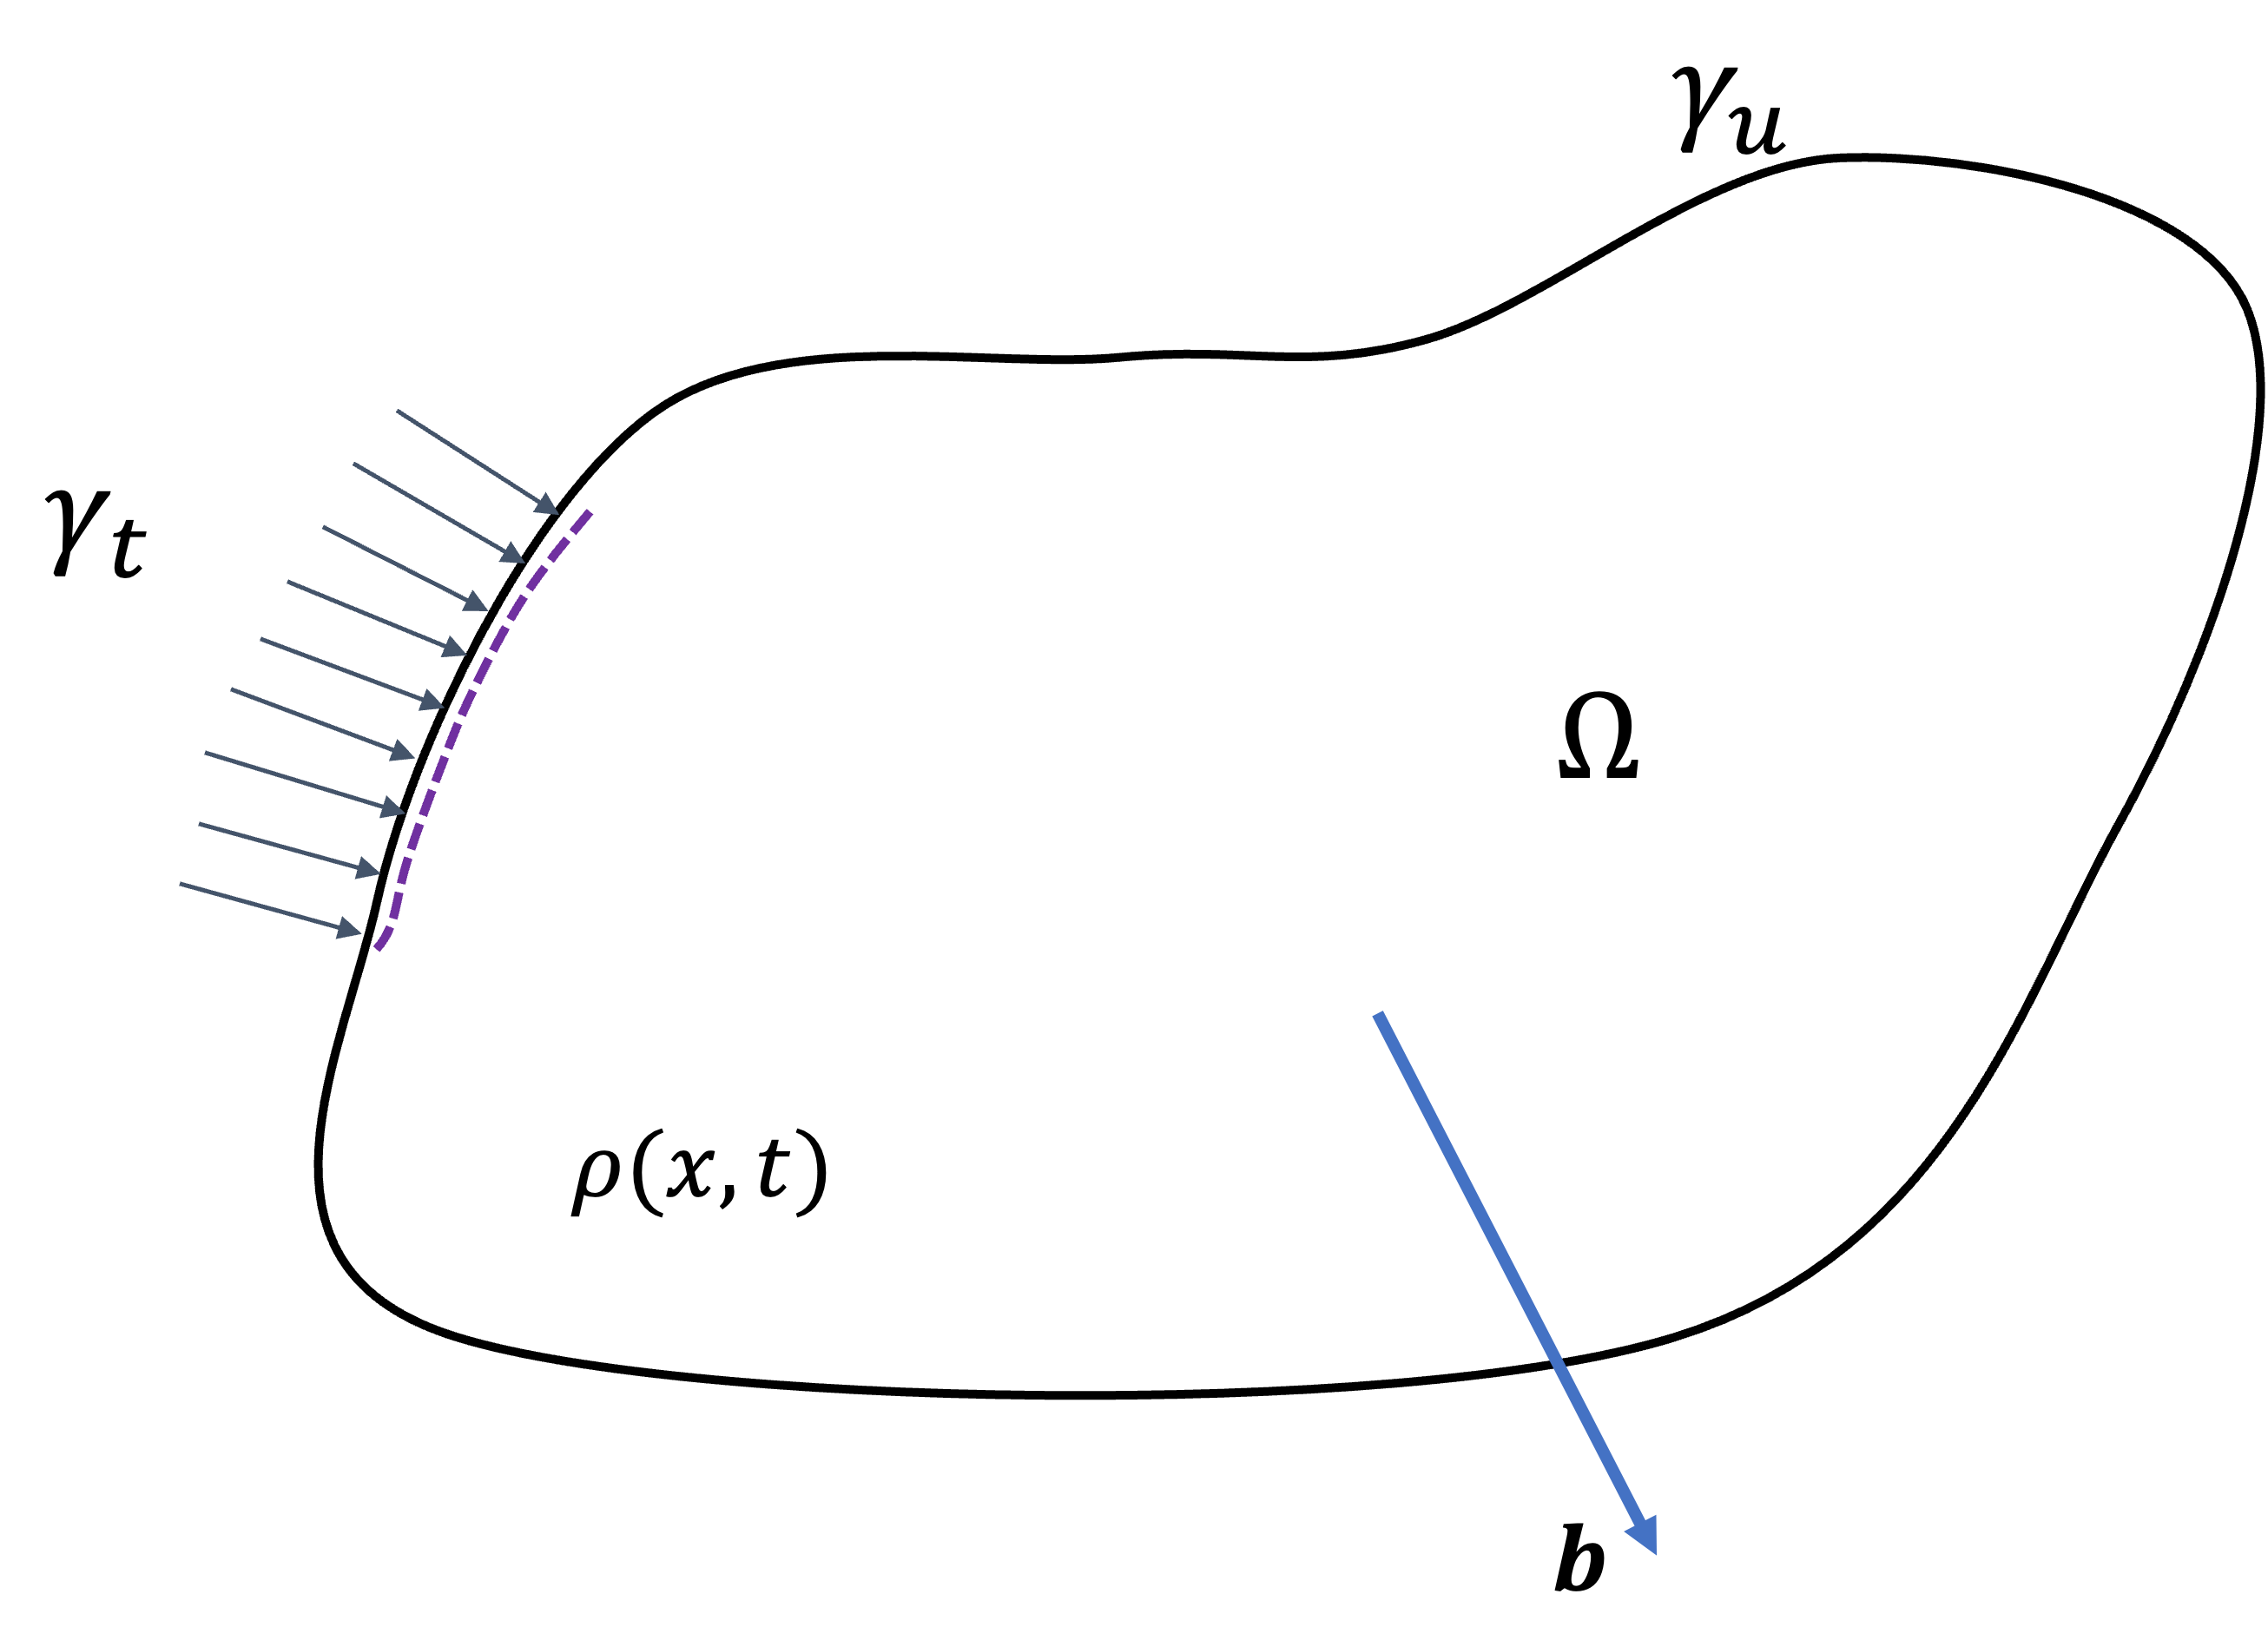
\includegraphics[width=0.4\textwidth]{./PICS/MPMEq.png}
\caption{Various stages in MPM computations}
\label{Fig:MPM_Dom}
\end{figure}
For a continuum body occupying a region $\Omega$ in space and bounded by a surface $\Gamma=\Gamma_u \cup \Gamma_t$ as shown in Figure~\ref{Fig:MPM_Dom}, the total mass $m$ of the body is given by,
\begin{align}
m=\int_{\Omega} \rho(\mathbf{x}, t) d V
\end{align}
where $\rho$ is the density of the material.

Since the mass contained in the region $\Omega$ and moving with local velocity is constant, the total time derivative is zero. Hence,
\begin{align}
\frac{\mathrm{D}}{\mathrm{D} t} \int_{\Omega} \rho(\mathbf{x}, t) \mathrm{d} V=\int_{\Omega}(\dot{\rho}+\rho \nabla \cdot \boldsymbol{v}) \mathrm{d} V=0
\end{align}

which leads to the mass conservation equation as,
\begin{align}
\rho J-\rho_0=0
\end{align}

\subsection{Conservation of momentum}
The Newton's second law of motion states that the rate of change of momentum of a body is equal to the sum of volume and surface forces acting on it. Consider the same body as shown in Figure~\ref{Fig:MPM_Dom}, with a body force per unit mass $\mathbf{b}$ and traction $\mathbf{t}$ acting on it's surface. The law of conservation of momentum is expressed as,
\begin{align}
\frac{\mathrm{D}}{\mathrm{D} t} \int_{\Omega} \rho \mathbf{v} \mathrm{d} V=\int_{\Omega} \rho \mathbf{b}(\mathbf{x},t) \mathrm{d} V + \int_{\Gamma_t} \mathbf{t}(\mathbf{x},t).\mathbf{n} \mathrm{d} A
\end{align}

By invoking the Reynolds transport theorum and upon simplifying one obtains,
\begin{align}
\rho \dot{\mathbf{v}} = \rho \mathbf{b} + \nabla . \sigma 
\end{align}


\subsection{Initial and Boundary conditions}
Two types of boundary conditions are considered in MPM solution, namely boundaries with specified velocity and specified traction respectively.
\begin{align}
& \left\{\begin{array}{l}
\left.(\boldsymbol{n} \cdot \boldsymbol{\sigma})\right|_{\Gamma_t}=\overline{\boldsymbol{t}} \\
\left.\boldsymbol{v}\right|_{\Gamma_u}=\overline{\boldsymbol{v}}
\end{array}\right. \\
\end{align}
Initial conditions in MPM involve specifying displacement of material points and velocities at time t=0.
\begin{align}
& \mathbf{v}(\mathbf{x}, 0)=\mathbf{v}_0(\mathbf{x}), \quad \mathbf{u}(\mathbf{x}, 0)=\mathbf{u}_0(\mathbf{x})
\end{align}


\section{Governing Equations of MPM}
%Flow of information to communicate to the reader
The full set of governing equations for the membrane compaction problem discussed in the previous section is summarized as,

\begin{align}
\rho J-\rho_0=0
\label{Eq:mce}
\end{align}

\begin{align}
\rho \dot{\mathbf{v}} = \rho \mathbf{b} + \nabla . \sigma
\end{align}

The equation ofconservation of mass is not solved explicitly. Instead it is used to calculate the updated density field in the computations through Eq.~\ref{Eq:mce}. Like in many finite-element formulations, the method of weighted residuals is used to reduce the residual (error) to zero in an average sense. By taking the virtual displacement $\delta u_j \in \Re_0, \Re_0=\left\{\delta u_j\left|\delta u_j \in C^0, \delta u_j\right|_{\Gamma_u}=0\right\}$ as the test function, one obtains the weak form of the governing equations and the traction boundary condition as,

\begin{align}
	\begin{array}{r}
\int_{\Omega} \delta u_i\left(\sigma_{i j, j}+\rho b_i-\rho \ddot{u}_i\right) \mathrm{d} V=0, \\
\int_{\Gamma_t} \delta u_i\left(\sigma_{i j} n_j-\bar{t}_i\right) \mathrm{d} V=0,
\end{array}
\end{align}

which upon simplification is shown below.

\begin{align}
\int_{\Omega} \rho \ddot{u}_i \delta u_i \mathrm{~d} V+\int_{\Omega} \rho \sigma_{i j}^s \delta u_{i, j} \mathrm{~d} V-\int_{\Omega} \rho b_i \delta u_i \mathrm{~d} V-\int_{\Gamma_t} \rho \bar{t}_i^s \delta u_i \mathrm{~d} A=0
\label{Eq:GovEqMPM}
\end{align}

In the standard formulation of MPM used in this study, the density field in the domain is approximated as,
\begin{align}
\rho(\boldsymbol{x})=\sum_{p=1}^{n_p} m_p \delta\left(\boldsymbol{x}-\boldsymbol{x}_p\right)
\label{Eq:rho_def}
\end{align}

In the above equation, ${n_p}$ is the number of material points. Substituting Eq.~\ref{Eq:rho_def} in Eq.~\ref{Eq:GovEqMPM} and invoking particle quadrature, one obtains the numerical governing equation of MPM.  

\begin{align}
\sum_{p=1}^{n_p} m_p \ddot{u}_{i p} \delta u_{i p}+\sum_{p=1}^{n_p} m_p \sigma_{i j p}^s \delta u_{i p, j}-\sum_{p=1}^{n_p} m_p b_{i p} \delta u_{i p}-\sum_{p=1}^{n_p} m_p \bar{t}_{i p}^s h^{-1} \delta u_{i p}=0
\label{Eq:NumEqMPM}
\end{align}
The subscipts $p$ and $i$ refer to the particle and spatial dimension respectively. The solution of the numerical governing equation above is carried out in four stages as briefly discussed in the following sub-sections.
\subsection{Particle to Grid Interpolation (P2G)}
In this step, the material points are assumed to be attached to the background grid as shown in Figure~\ref{Fig:MPM_Steps}(a). The background grid is then considered similar to a finite element grid and based on the shape function defined at the grid node $I$ the unknown quantities in Eq.~\ref{Eq:NumEqMPM} are calculated as,
\begin{align}
\begin{array}{r}
u_{i p}  =N_{I p} u_{i I} \\
u_{i p, j}  =N_{I p, j} u_{i I}\\
\delta u_{i p} =N_{I p} \delta u_{i I}
\end{array}
\label{Eq:shape}
\end{align} 
In the equations above, subscript $I$ is used to denote the grid node and $N_I$ indicate the shape function defined at node $I$. In this study, two shape functions namely, the linear-hat and cubic spline shape functions are considered.
Substituting equations Eq.~\ref{Eq:shape} in Eq.~\ref{Eq:NumEqMPM} and cancelling the common virtual displacement term $\delta u_{i I}$, one obtains,
\begin{align}
m_{I J} \dot{u}_{i J}=f_{i I}^{\mathrm{int}}+f_{i I}^{\mathrm{ext}}, \quad x_I \notin \Gamma_u
\end{align} 

where $m_{I J}$ is the elements of the mass matrix defined as,
\begin{align}
m_{I J}=\sum_{p=1}^{n_p} m_p N_{I p} N_{J p}\\
\end{align}
 
and $f_{i I}^{\mathrm{int}}$ and $f_{i I}^{\mathrm{ext}}$ are the internal and external forces respectively and given by,
\begin{align}
f_{i I}^{\mathrm{int}}=-\sum_{p=1}^{n_p} N_{I p, j} \sigma_{i j p} \frac{m_p}{\rho_p} \\
f_{i I}^{\mathrm{ext}}=\sum_{p=1}^{n_p} m_p N_{I p} b_{i p}+\sum_{p=1}^{n_p} N_{I p} \bar{t}_{i p} h^{-1} \frac{m_p}{\rho_p}
\end{align}
Hence, this step of the MPM solution procedure involves 'projecting' properties from  material points to grid nodes and is shown schematically in Figure~\ref{Fig:MPM_Steps}(a).

\subsection{Temporal integration at grid nodes}
Once the grid nodal properties are calculated in the P2G operation, the updated velocity at grid nodes are calculated. In this study, a simple forward Euler time integration procedure is used. Since this procedure in its original form involves costly inversion of the mass matrix $m_{I J}$, the following mass-lumping approximation is made,

\begin{align}
m_I=\sum_{J=1}^{n_g} m_{I J}=\sum_{p=1}^{n_p} m_p N_{I p}
\end{align}

The velocity components at the nodes are then calculated as,
\begin{align}
\mathbf{v_{I}}^{t+\Delta t}=\mathbf{v_{I}}^{t}+\frac{1}{m_I} \left(\mathbf{f_{i I}}^{\mathrm{int}}+\mathbf{f_{i I}}^{\mathrm{ext}}\right)
\end{align}

where $\Delta t$ is the time step used in time integration and is calculated from the following equation,
\begin{align}
\Delta t= CFL \min \left(\frac{h_x}{c_x}, \frac{h_y}{c_y}, \frac{h_z}{c_z}\right)
\end{align}

Here, $c_()$ and $h_()$ refer to characteristic velocity and grid sizes in different directions respectively.

\subsection{Grid to Particle (G2P) Interpolation}
Once the updated velocities at grid nodes are obtained, the velocities and their gradients at the material points are obtained in this step as, 

\begin{align}
\mathbf{v}_p^{t+\Delta t}=\alpha_{P-F}\left(\mathbf{v}_p^t+\sum_I N_I \left[{\mathbf{v}}_I^{t+\Delta t}-\mathbf{v}_I^t\right]\right)+(1-\alpha_{P-F}) \sum_I N_I {\mathbf{v}}_I^{t+\Delta t}\\
\nabla \mathbf{v}_p^{t+\Delta t}=\sum_I^{ng} \nabla N_I \mathbf{v}_I^{t+\Delta t}
\end{align}

The term $\alpha_{P-F}$ used in the material point velocity update step above determines the level of blending between Particle-in-Cell (PIC) and Fluid Implicit Particle Method (FLIP) like updates.
The velocity gradient thus calculated at the material point is used to compute the stress tensor through the user-provided constitutive relation. 

\subsection{Material point position update and grid reset}
At this step, the updated velocity at the material point is already obtained and is used to update the material point position as,
\begin{align}
\mathbf{x}_{p}^{t+\Delta t}=\mathbf{x}_{p}^{t} +\Delta t \: \mathbf{v}_p^{t+\Delta t}
\end{align}

The background grid in MPM is used only as a scratch pad to calculate gradients and for time integration and hence is often reset or regenerated at the end of each MPM step.


\begin{figure}[h]
\subfloat[Particle to grid (P2G) operation]{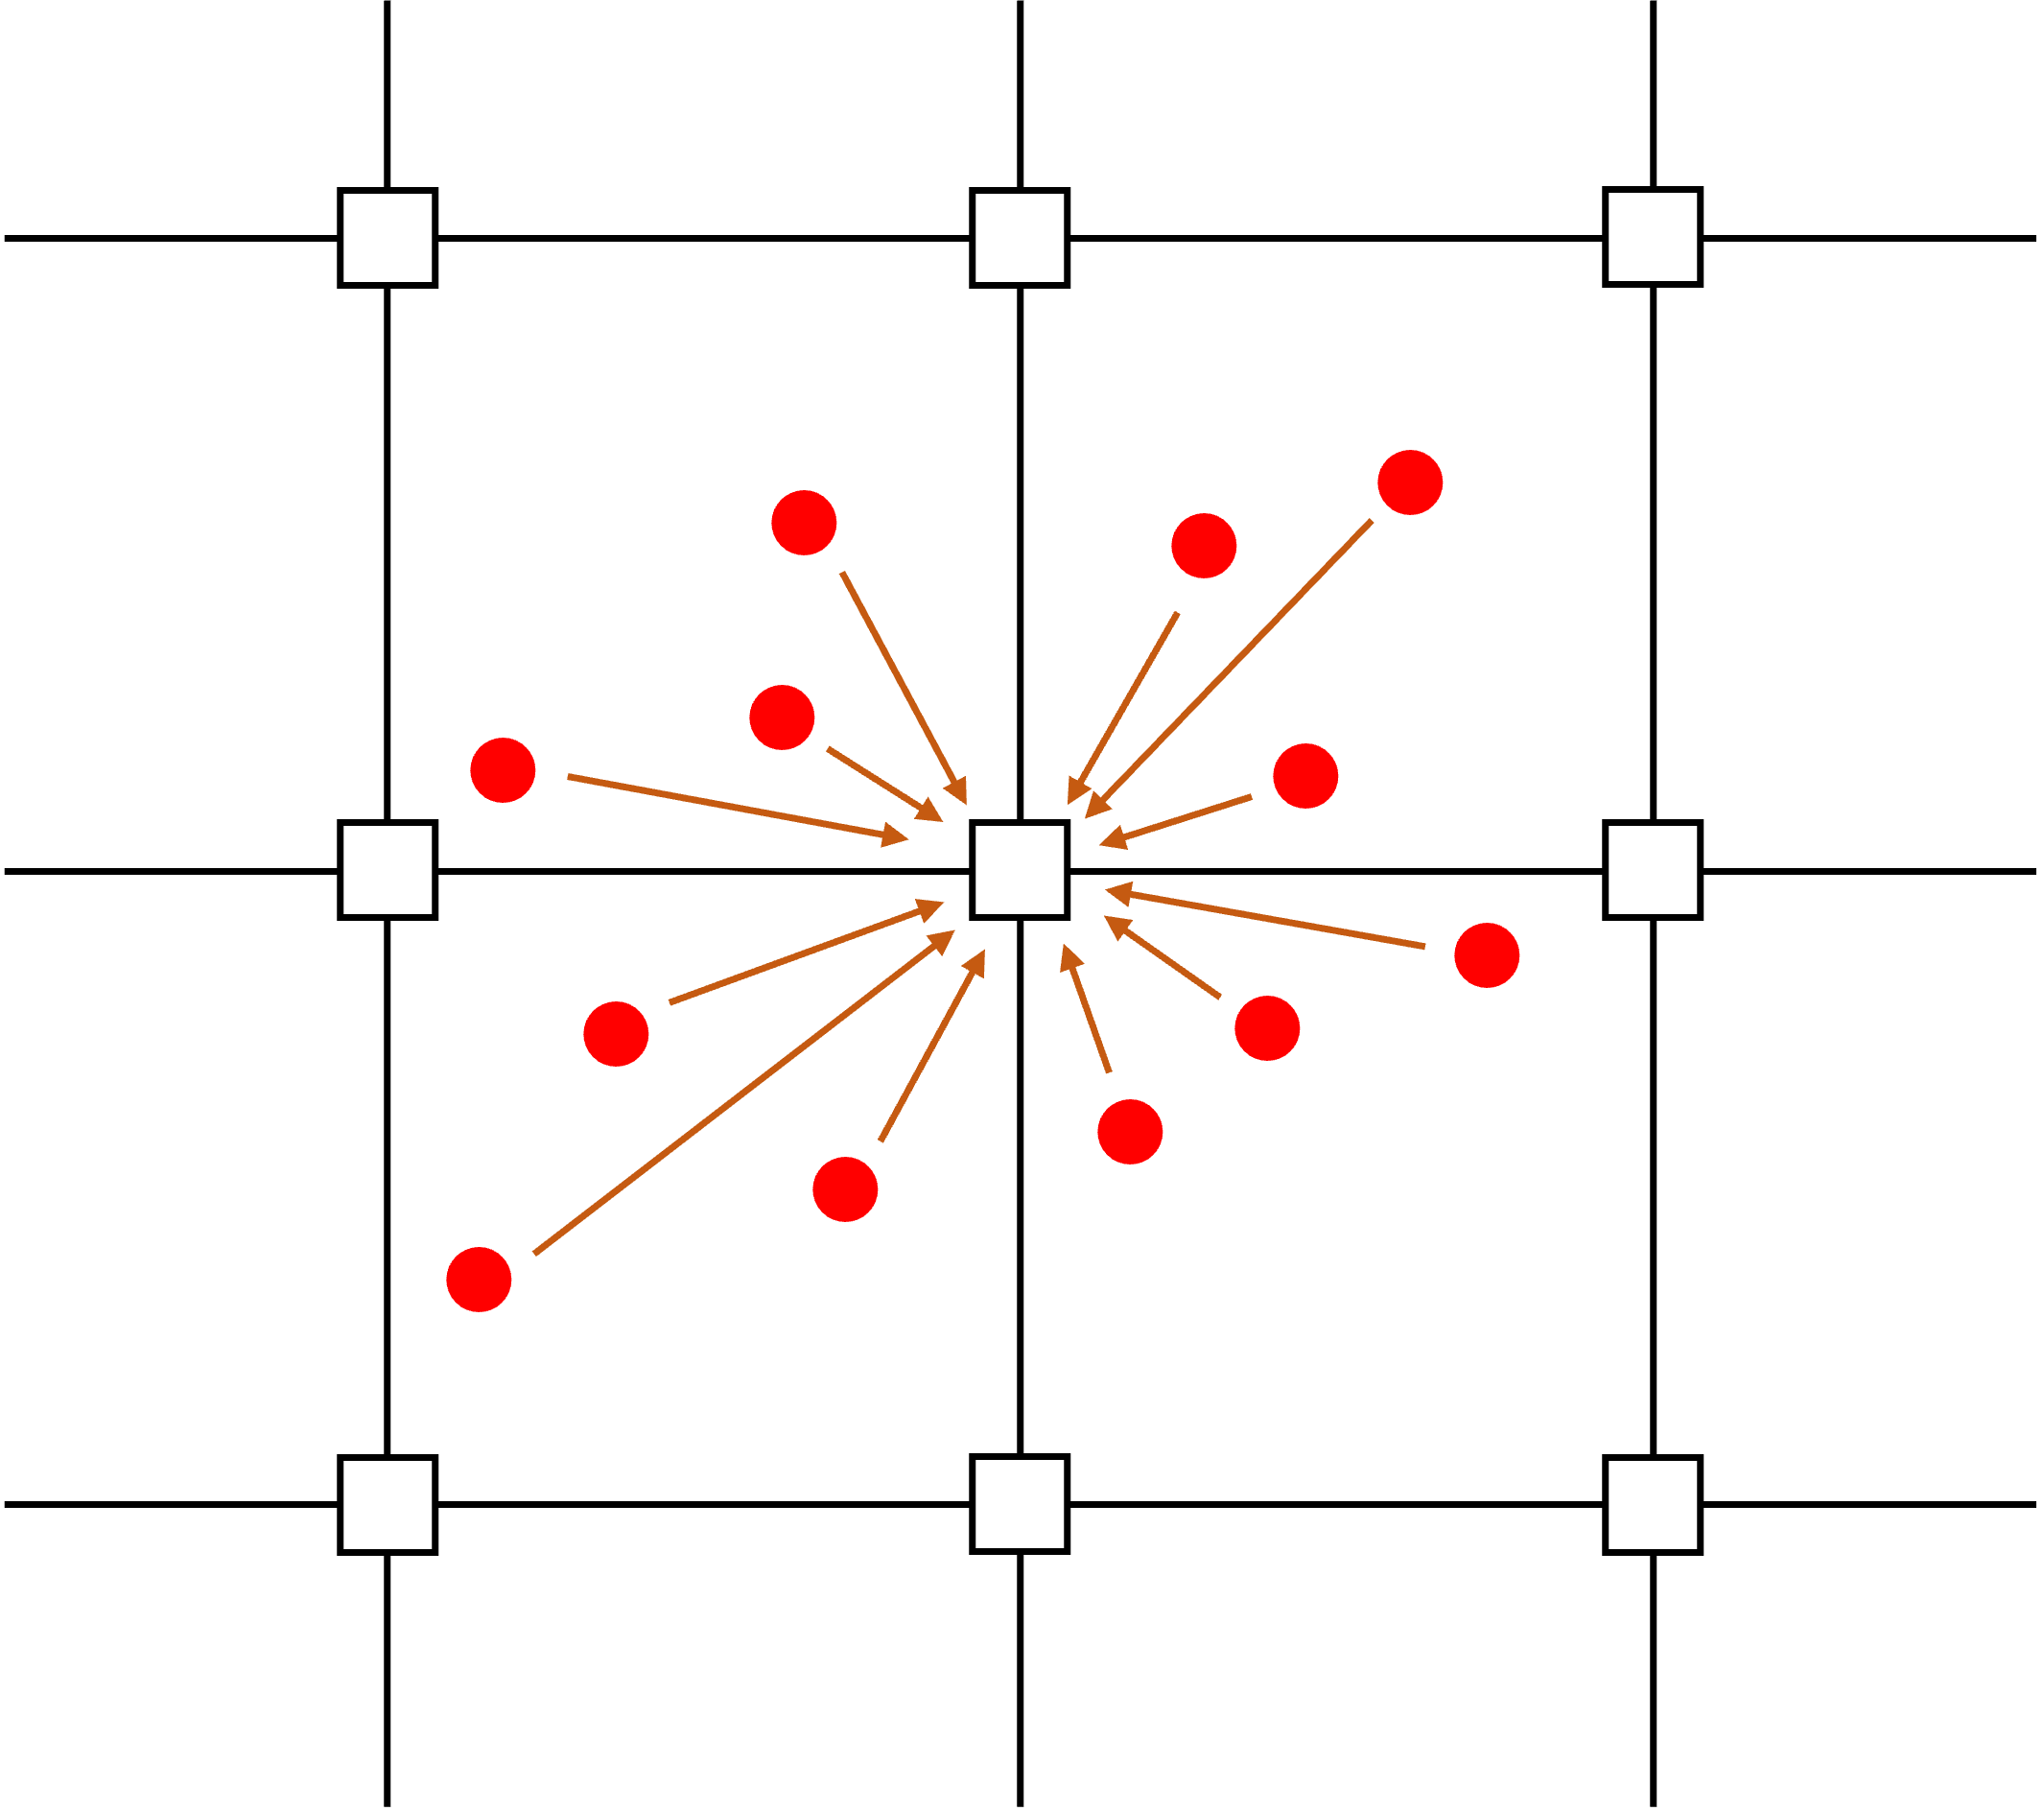
\includegraphics[width=0.4\textwidth]{./PICS/MPM_Step1.png}}
\subfloat[Nodal velocity update]{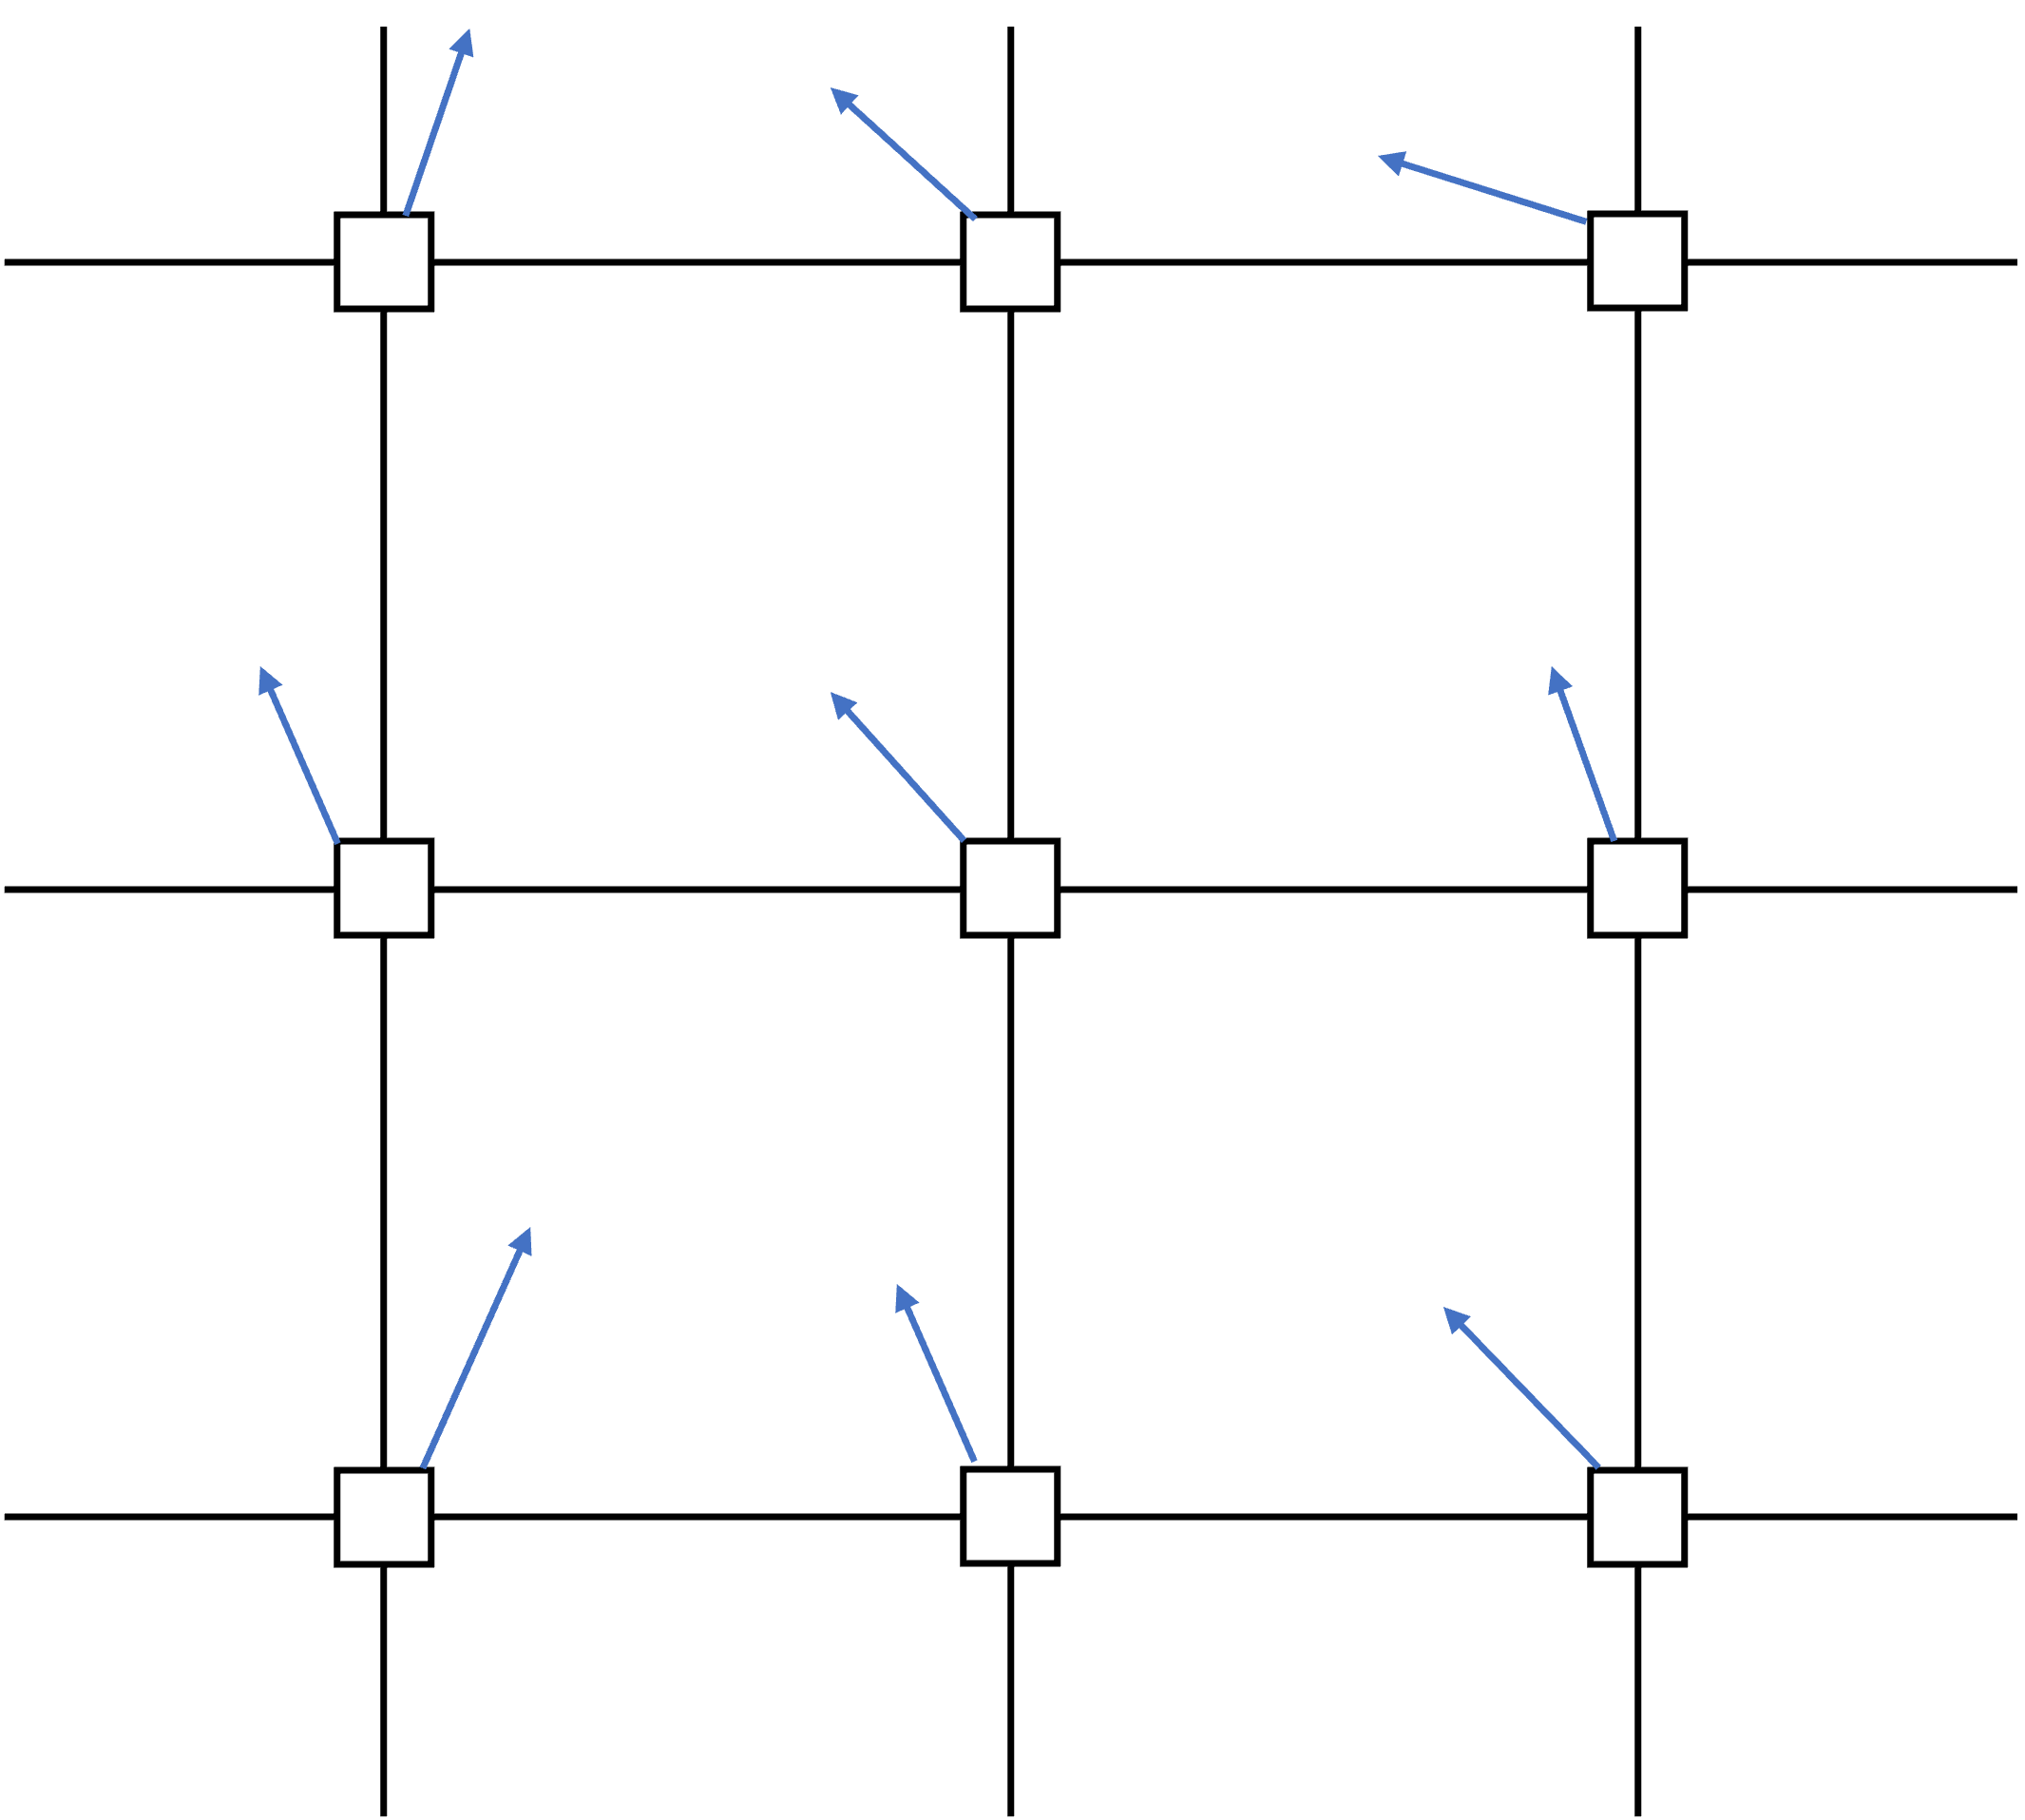
\includegraphics[width=0.4\textwidth]{./PICS/MPM_Step2.png}}\\
\subfloat[Grid to particle (G2P) operation]{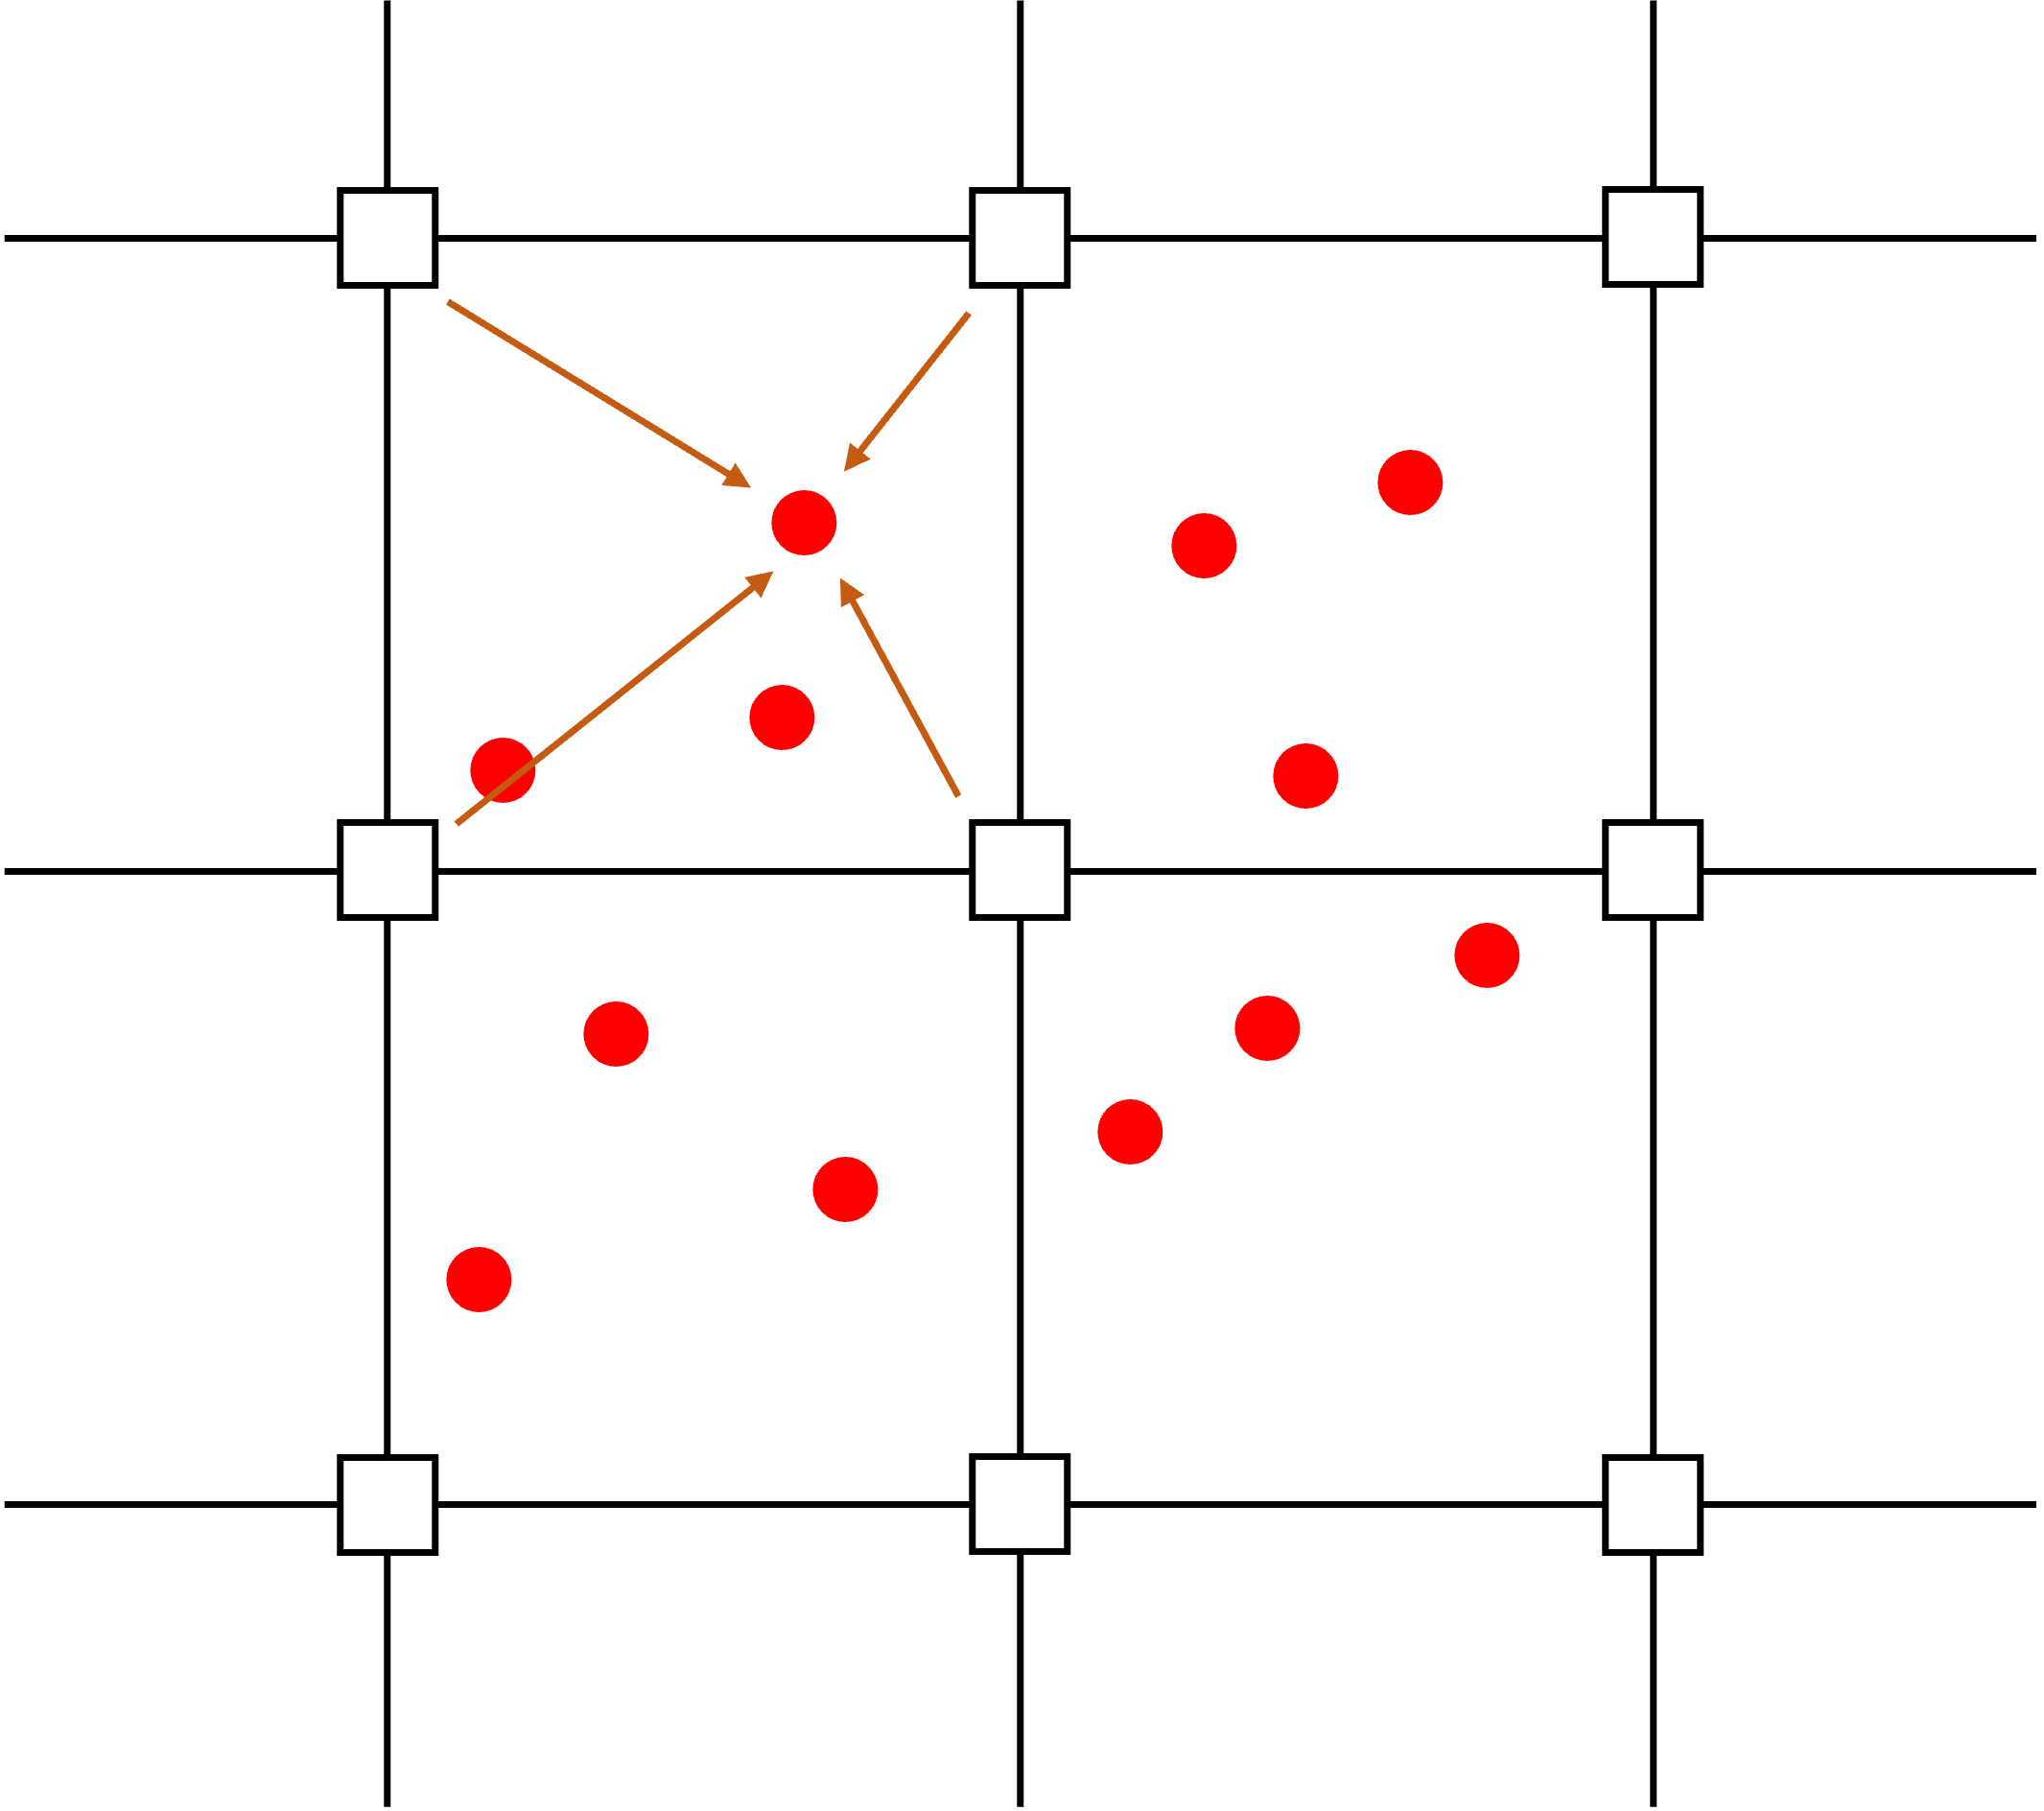
\includegraphics[width=0.4\textwidth]{./PICS/MPM_Step4.png}}
\subfloat[Particle position update]{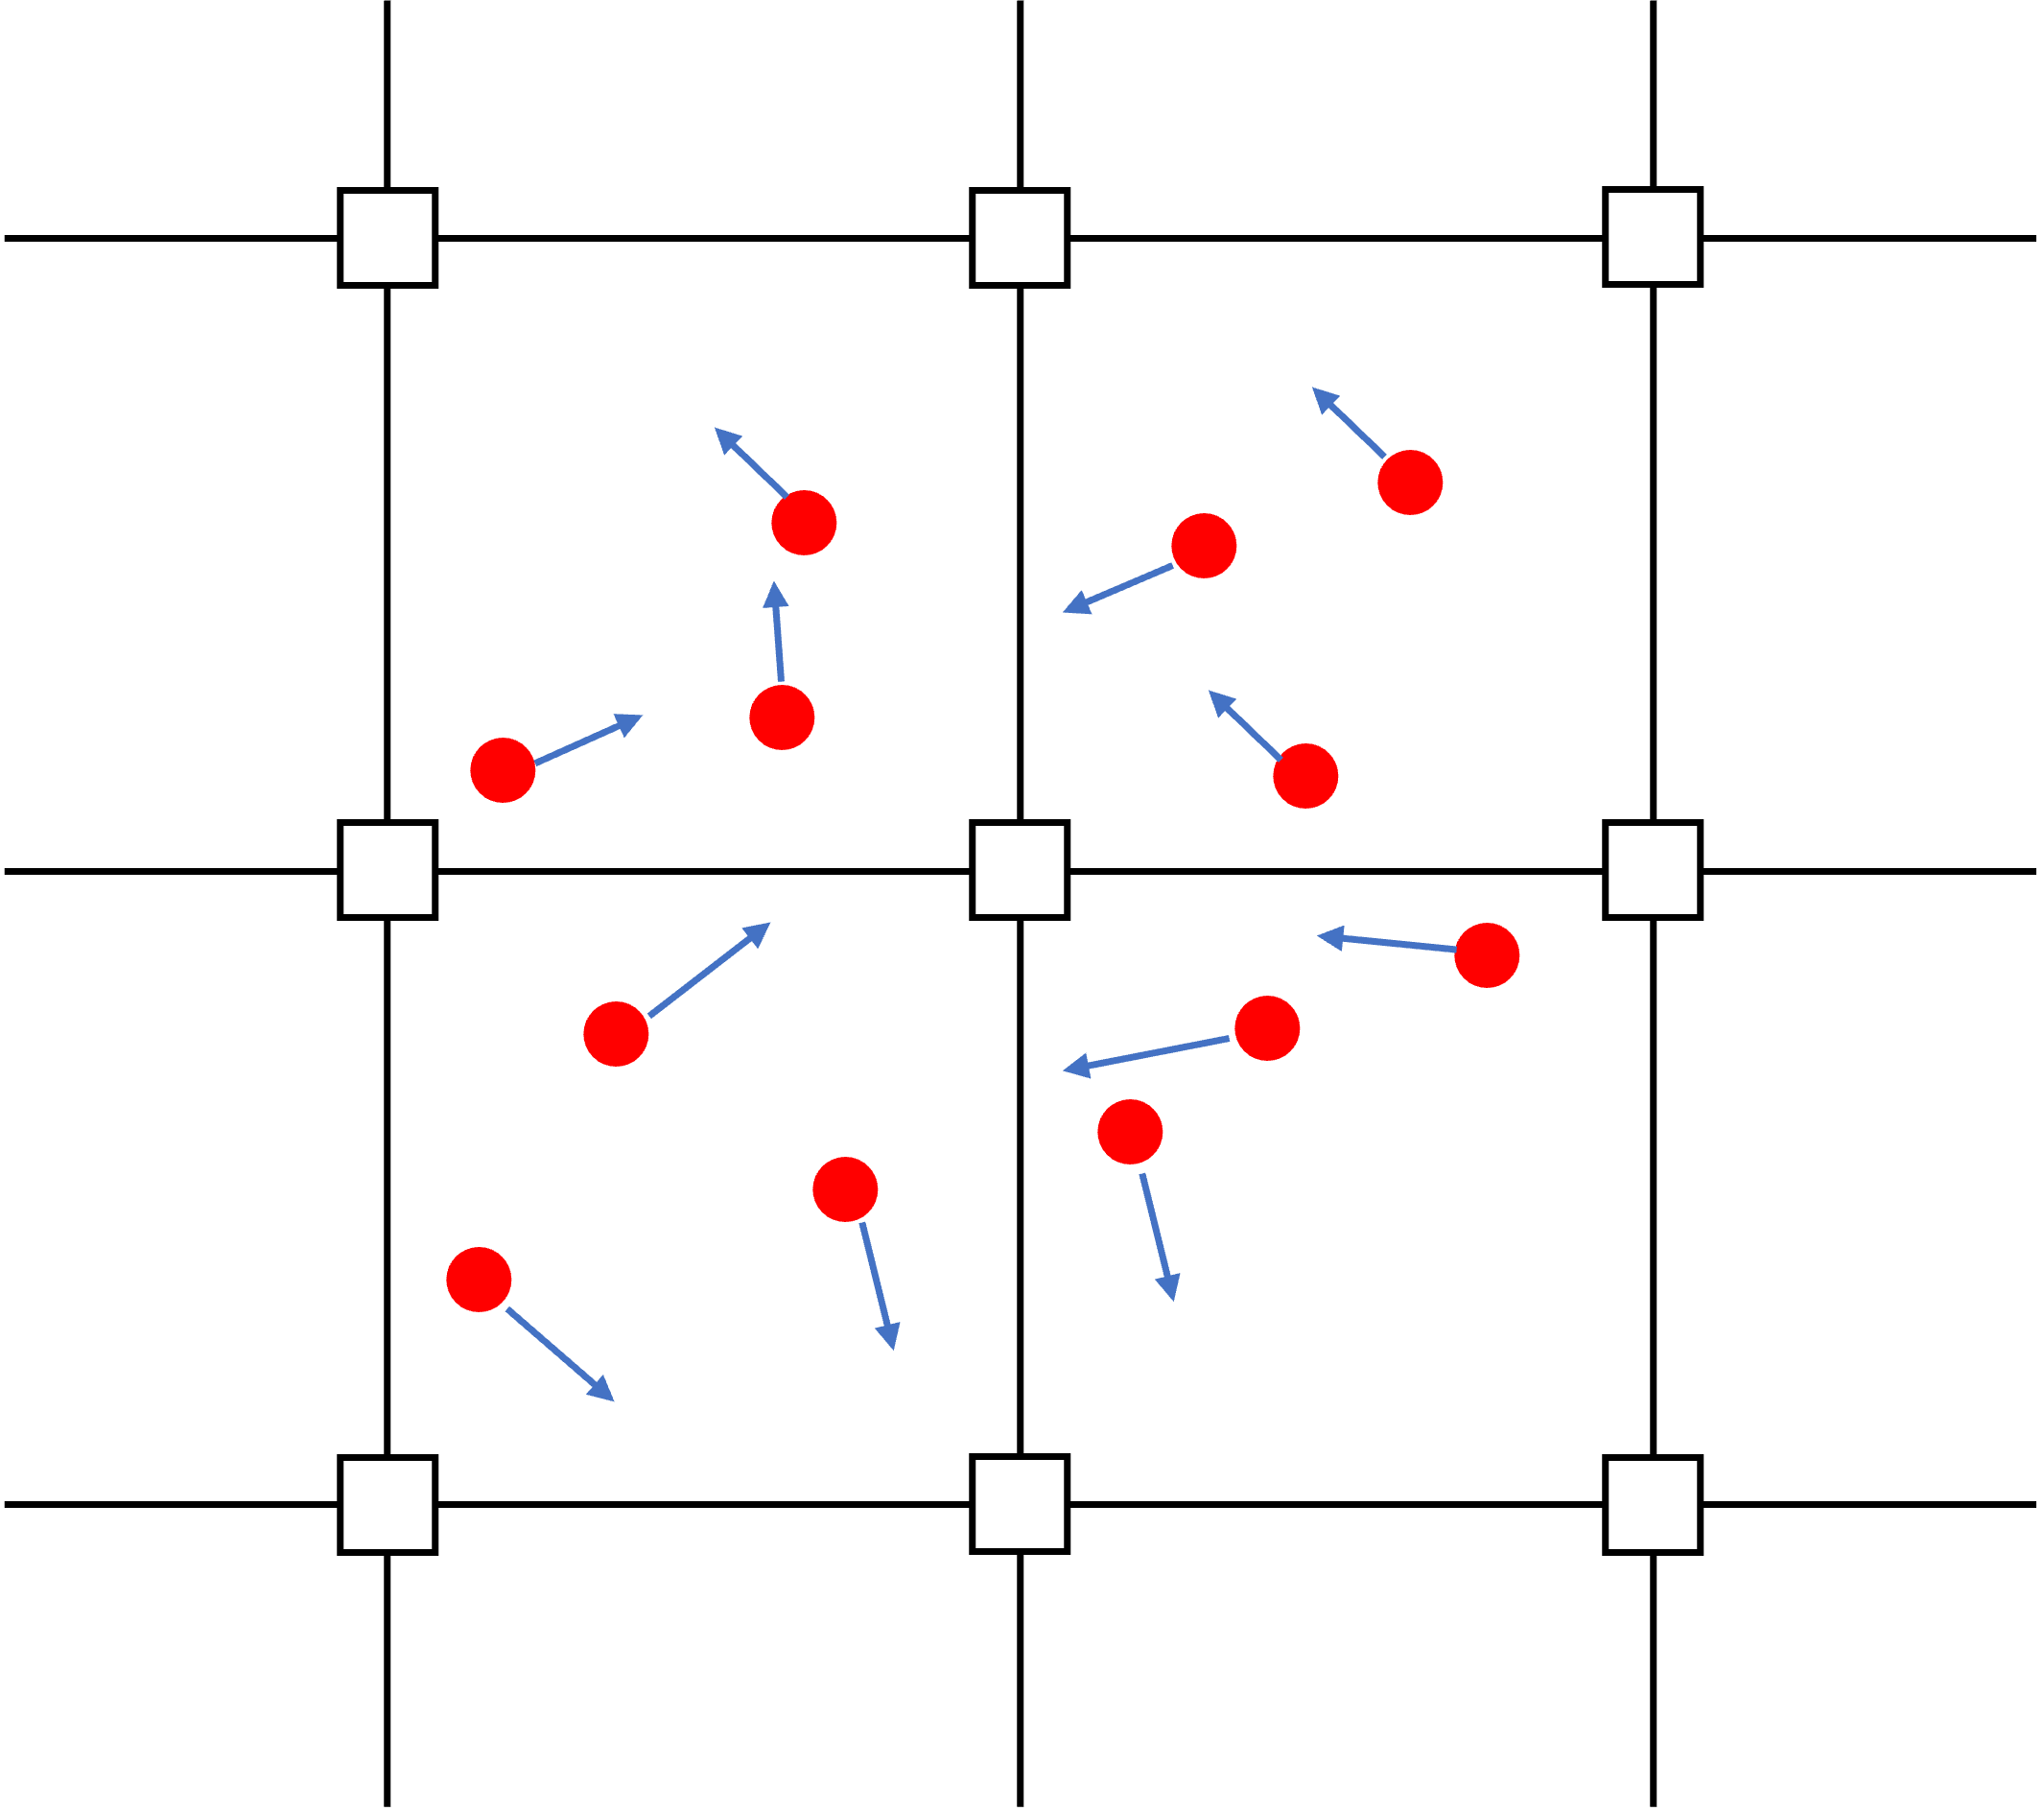
\includegraphics[width=0.4\textwidth]{./PICS/MPM_Step3.png}}
\caption{Various stages in MPM computations. The square symbols and associated lines indicate grid nodes and cell edges respectively. The background grid in most MPM codes is cartesian due to ease of grid generation. The red circles indicate material points}
\label{Fig:MPM_Steps}
\end{figure}
\section{MPM Validation}
The formulation discussed in the previous section is used to develop the MPM Solver \Ex. \Ex is developed at the HPACF team at the National Renewable Energy Lab and is available publically as a Github repository (https://github.com/NREL/Exagoop).
The \Ex  MPM solver is validated and verified on a multitude of test cases of which three are presented in the following subsections.

\subsection{Axial vibration of bar}
In this test case, the axial free vibration of a continuum bar made of a linearly elastic material is studied. This is one of the test cases for which the exact solution is known. 
\begin{figure}[h]
\subfloat[]{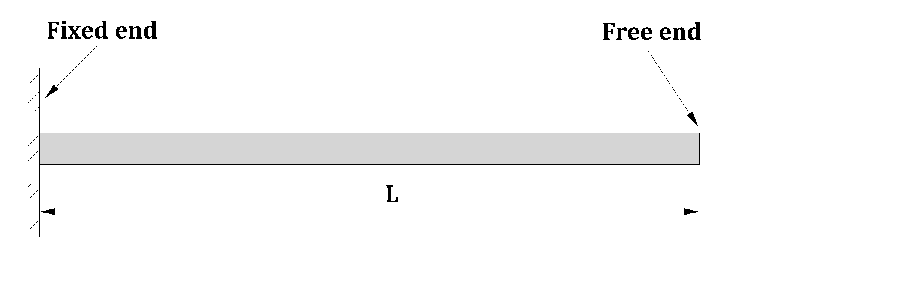
\includegraphics[width=0.6\textwidth]{./PICS/AxBar_PDT.pdf}}\\
\subfloat[]{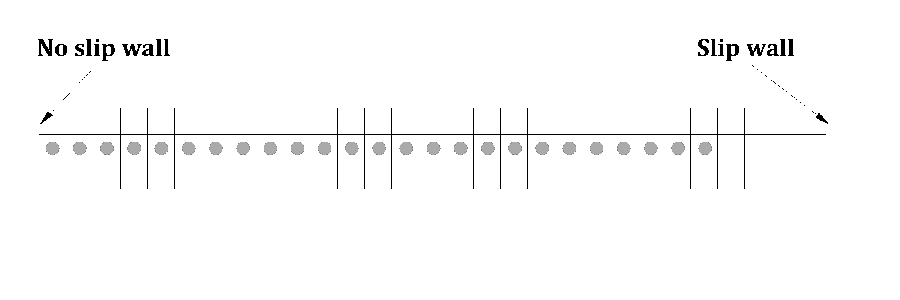
\includegraphics[width=0.6\textwidth]{./PICS/AxBar_PDMPM.pdf}}
\caption{Axial vibration of bar. (a) Configuration of test case (b) Corresponding MPM modeling. Gray lines indicate the background Eulerian grid and the gray circles are the material points located at time $t=0$}
\label{Fig:TestCaseAxBar}
\end{figure}
The test case configuration is shown in Figure~\ref{Fig:TestCaseAxBar}(a). The bar has a length $L$ with an area of cross-section $A$ and is made up of a linear elastic material with Young's modulus $E$. The poisson's ratio of the material is set as zero. The bar is fixed at one end and left free at the other. The equation governing the vibration of the bar is given by,
\begin{align}
	\frac{\partial^2 u}{\partial t^2}=c^2 \frac{\partial^2 u}{\partial x^2}
\label{Eq:goveq_axial_bar}
\end{align}
where $u$ is the axial displacement and $c$ is the speed of sound in the elastic medium. The bar is subjected to the following boundary conditions as previously explained. 
\begin{align}
	u(0,t)=0\\
	\frac{\partial u}{\partial x} (L,t) = 0
\end{align}
When an initial axial velocity $v(x,0)= V_0 \sin \left(\frac{\pi x}{2 L}\right)$ is imposed on the bar, the full exact solution to the governing equation Eq~\ref{Eq:goveq_axial_bar} is given by,
\begin{align}
& u(x, t)=\frac{V_0}{\omega_1} \sin \left(\frac{\pi x}{2 L}\right) \sin \left(\omega_1 t\right) \\
& v(x, t)=V_0 \sin \left(\frac{\pi x}{2 L}\right) \cos \left(\omega_1 t\right)
\end{align}
where $\omega_1$ is the fundamental frequency of the first mode of vibration.
%Explanation on the numerical set up.

Numerical simulations of this test case is performed using \Ex solver. The properties of the bar are set as $E=100, L=25$ and $V_0 = 0.1$.  The density of the material, $\rho$ is set equal to unity. The length of the bar is descretized using $25$ material points located equidistant from each other. A three-dimensional, structured background grid is chosen in this study with grid edge of unit length.  The grid has three cells each in both the lateral dimensions and $29$ grid cells in the longitudinal direction such that at the initial time each material point is located at the center of the cell as shown in Figure~\ref{Fig:TestCaseAxBar}(b). Four grid cells are left as a buffer region between the right most material point and the right boundary of the background grid. No-slip and slip wall boundary conditions are imposed on the left and the right boundaries respectively while periodic boundary conditions are imposed in the other directions. Simulations are performed using both the linear-hat shape functions as well as the cubic-spline shape functions and for $\alpha_{P-F}$ equal to zero and one respectively. The CFL numbers are also varied $0.01$ to $0.5$ in different simulations. For ease of presentation, the comparisons between the exact solution and the MPM solutions obtained using \Ex are shown here using the center of mass velocity of the bar, $v_{cm}$ and using system energies. The exact center of mass velocity is given by $v_{\mathrm{cm}}^{\mathrm{exa}}(t)=\frac{V_0 c}{\omega_1 L} \cos \left(\omega_1 t\right)$ and its MPM counterpart is calculated as $v_{\mathrm{cm}}^{\mathrm{num}}(t)=\frac{\sum v_p(t) m_p}{\sum m_p}$. Three different forms of system energy is shown for comparison, namely the kinetic energy ($KE=\frac{1}{2} \sum_{p=1}^{n_p} \mathbf{v}_p \cdot \mathbf{v}_p m_p$), the strain energy ($SE=\frac{1}{2} \sum_{p=1}^{n_p} \sigma_{p} \epsilon_{p} V_p$) and the total energy ($TE=KE+SE$).

\subsubsection{Effect of $\alpha_{P-F}$}
Figure~\ref{Fig:TestCaseAxBar_EoA_Vel} shows the variation of $v_{cm}$ as a function of time for two different values of $\alpha_{P-F}$ ($0$ and $1$). It is observed that for $\alpha_{P-F}=0$, the center of mass velocity decreases with time in contrast to the exact solution where the amplitude remains unchanged. On the other hand, for $\alpha_{P-F}=1$ the exact nature of the solution is well captured by MPM solution.

\begin{figure}[h]
\subfloat[$\alpha_{P-F}=0$]{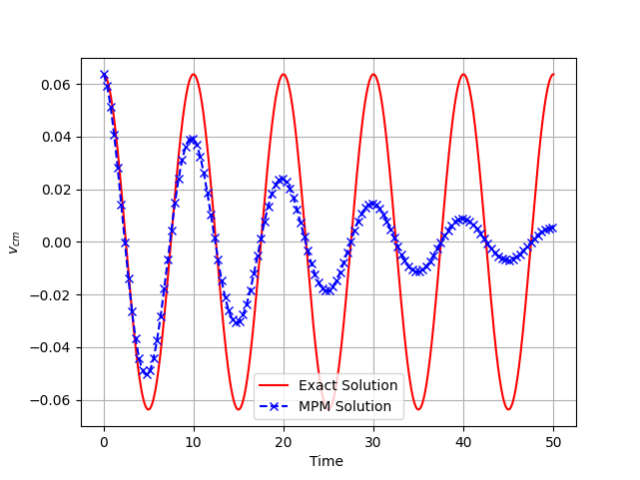
\includegraphics[width=0.4\textwidth]{./PICS/AVB_Effect_of_alpha_Vel_1Order_a=0.png}}
\subfloat[$\alpha_{P-F}=1$]{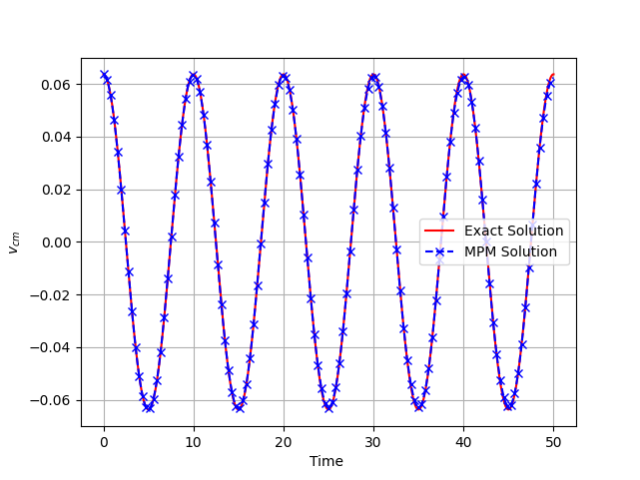
\includegraphics[width=0.4\textwidth]{./PICS/AVB_Effect_of_alpha_Vel_1Order_a=1.png}}
\caption{Exact and MPM computed center of mass velocity $v_{cm}$ as a function of time. Linear hat shape function used with $CFL=0.1$}
\label{Fig:TestCaseAxBar_EoA_Vel}
\end{figure}

This dissipative nature of the numerical solution at low values of $\alpha_{P-F}$ can also be observed from the temporal variation of energy plotted in Figure~\ref{Fig:TestCaseAxBar_EoA_Engy}. Both kinetic and strain energy (and hence the total energy as well) is found to decrease and ultimately reach zero with time for $\alpha_{P-F}=0$ while $\alpha_{P-F}=1$ captures the non-dissipative nature of the exact solution accurately.

\begin{figure}[h]
\subfloat[$\alpha_{P-F}=0$]{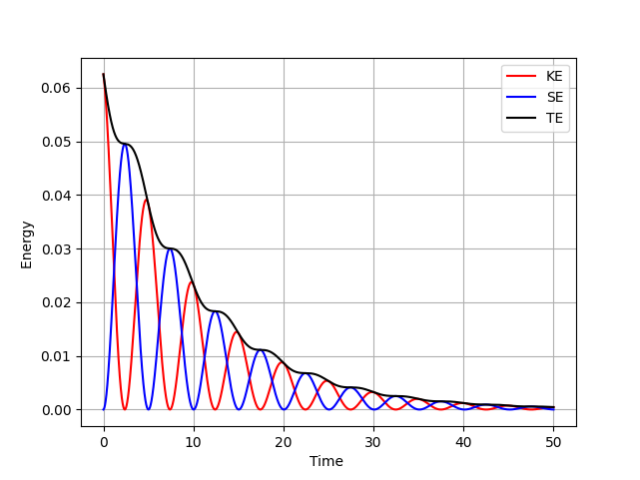
\includegraphics[width=0.3\textwidth]{./PICS/AVB_Effect_of_alpha_Engy_1Order_a=0.png}}
\subfloat[$\alpha_{P-F}=1$]{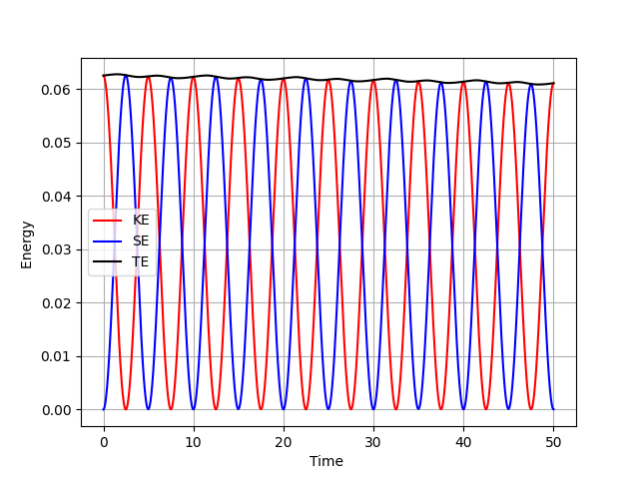
\includegraphics[width=0.3\textwidth]{./PICS/AVB_Effect_of_alpha_Engy_1Order_a=1.png}}
\caption{Exact and MPM computed energy  as a function of time. Linear hat shape function used with $CFL=0.1$}
\label{Fig:TestCaseAxBar_EoA_Engy}
\end{figure}

\subsubsection{Effect of $CFL$}
It is also interesting to study the effect of $CFL$ on the solution accuracy. Figure~\ref{Fig:TestCaseAxBar_EoCFL_CS_a0} shows the time evolution of $v_{cm}$ for values of $CFL=0.01,0.1$ and $0.5$. The results shown are obtained using the cubic spline shape functions and for $\alpha_{P-F}=0$. It is observed that the MPM solution deviates from the exact one as the $CFL$ is reduced. The solution is observed to be more dissipative as the CFL number is reduced. Results obtained using the linear hat shape function also show a similar trend and hence are not shown here.

\begin{figure}[h]
\subfloat[$CFL=0.01$]{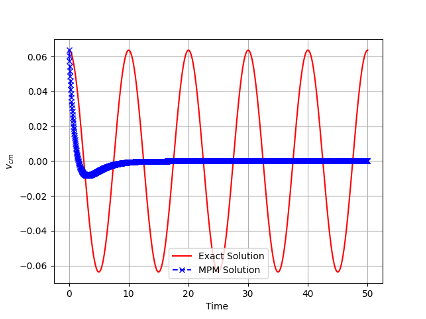
\includegraphics[width=0.3\textwidth]{./PICS/AVB_Effect_of_CFL_Vel_3Order_a=0_CFL_0p01.png}}
\subfloat[$CFL=0.1$]{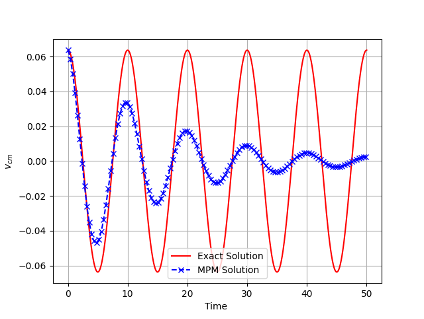
\includegraphics[width=0.3\textwidth]{./PICS/AVB_Effect_of_CFL_Vel_3Order_a=0_CFL_0p1.png}}
\subfloat[$CFL=0.5$]{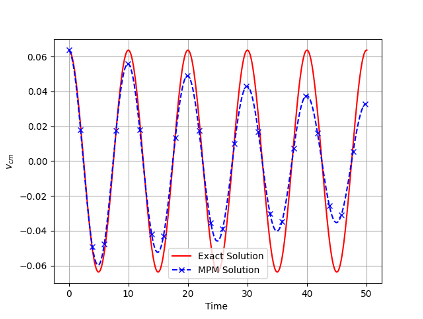
\includegraphics[width=0.3\textwidth]{./PICS/AVB_Effect_of_CFL_Vel_3Order_a=0_CFL_0p5.png}}
\caption{Exact and MPM center of mass velocity $v_{cm}$ as a function of time computed using cubic spline shape function.$\alpha_{P-F}=0$}
\label{Fig:TestCaseAxBar_EoCFL_CS_a0}
\end{figure}

On the contrary, very minimal deviations from exact solution are observed for all $CFL$ numbers for  $\alpha_{P-F}=1$ as shown in Figure~\ref{Fig:TestCaseAxBar_EoCFL_CS_a1}. Same trend also holds for solution computed using the linear hat shape function as well.

\begin{figure}[h]
\subfloat[$CFL=0.01$]{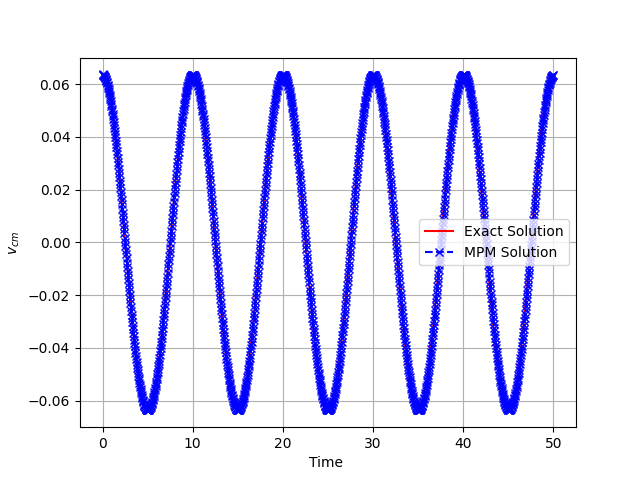
\includegraphics[width=0.3\textwidth]{./PICS/AVB_Effect_of_CFL_Vel_3Order_a=1_CFL_0p01.png}}
\subfloat[$CFL=0.1$]{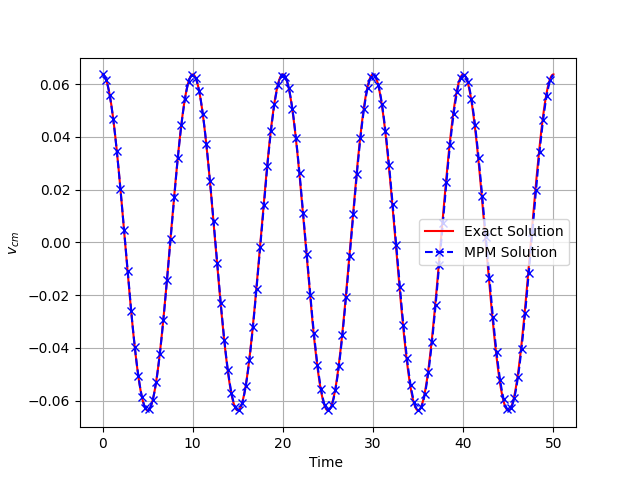
\includegraphics[width=0.3\textwidth]{./PICS/AVB_Effect_of_CFL_Vel_3Order_a=1_CFL_0p1.png}}
\subfloat[$CFL=0.5$]{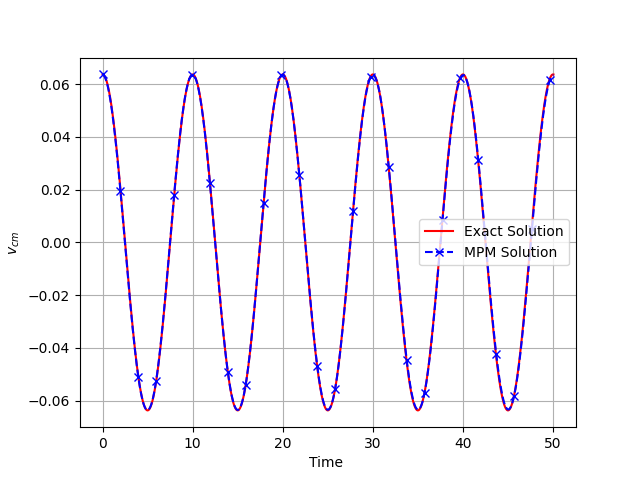
\includegraphics[width=0.3\textwidth]{./PICS/AVB_Effect_of_CFL_Vel_3Order_a=1_CFL_0p5.png}}
\caption{Exact and MPM center of mass velocity $v_{cm}$ as a function of time computed using cubic spline shape function.$\alpha_{P-F}=1$}
\label{Fig:TestCaseAxBar_EoCFL_CS_a1}
\end{figure}

Hence, it is concluded that lower values of $\alpha_{P-F}$ lead to dissipative solution. The dissipative nature further worsens for smaller values of CFL number as well. Hence, for all MPM simulations a typical value of $\alpha_{P-F}=0.95-1.0$ is used.


\subsection{Collision of two-dimensional elastic disks}
This test case is used to verify the \Ex capability to detect and simulate problems with collision. This two-dimensional test case configuration is shown in Figure~\ref{Fig:TestCaseEDC}(a) and consists of two elastics disks each of radius $r$ and separated by a distance $d$. At time $t=0$, both the disks have a velocity $v$ and move towards each other. As time progresses both the disks approach closer to each other at constant velocity and collide. After collision, the disks rebound and move away from each other. Since the collision is elastic, the total energy of the disks remain constant in time.

For simulating this test case in \Ex, the value of Young's modulous $E$ and density $\rho$ is chosen as $1000$. The poissons ratio is set as 0.3. The radius of the disks is set to 0.2 m each and the disks are separated by a distance $d=0.6\sqrt{2}$. The background grid is a square grid of side $L=2$m and consists of 20 cells each in the x and y directions. The two disks are modeled using linear elastic material points with four of them located inside each cell. Simulations are carried out using both the linear hat and the cubic spline shape functions. Based on the conclusions from the previous test case, the value of CFL and  $\alpha_{P-F}$ is chosen as 0.1 and 0.95 respectively. 

\begin{figure}[h]
\subfloat[]{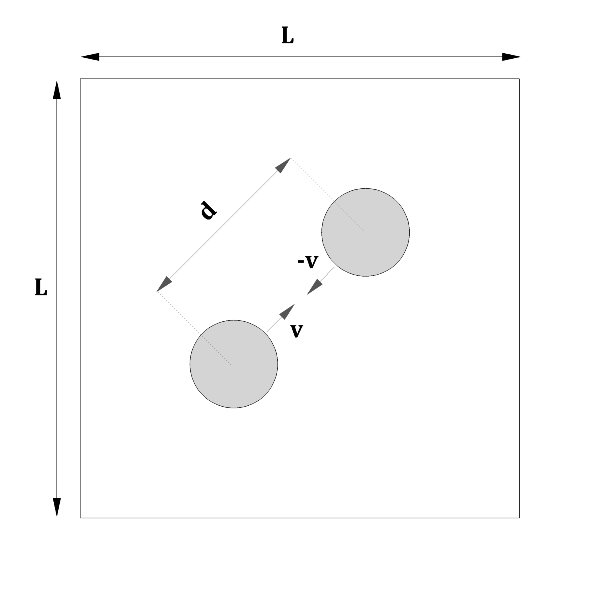
\includegraphics[width=0.35\textwidth]{./PICS/EDC_PDT.pdf}}
\subfloat[]{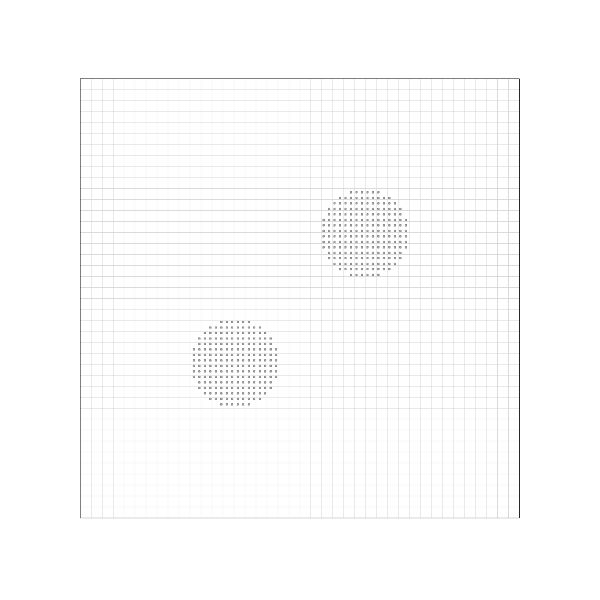
\includegraphics[width=0.35\textwidth]{./PICS/EDC_PDMPM.pdf}}
\caption{(a) Problem definition of the elastic collision of disks test case. (b) MPM background grid and disks modeled through material points}
\label{Fig:TestCaseEDC}
\end{figure}

Figures~\ref{Fig:TestCaseEDC_Res1}(a) and (b) show the approach of the disks towards each other.  Figures~\ref{Fig:TestCaseEDC_Res1}(c) shows the instant at which the disks collide and (d) shows the disks rebounding after collision. 

\begin{figure}[h]
\subfloat[$t=0$]{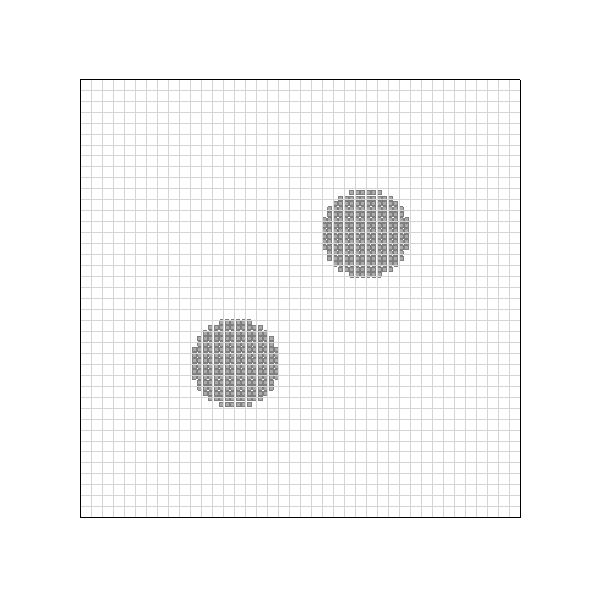
\includegraphics[width=0.2\textwidth]{./PICS/EDC1.pdf}}
\subfloat[$t=0.85$]{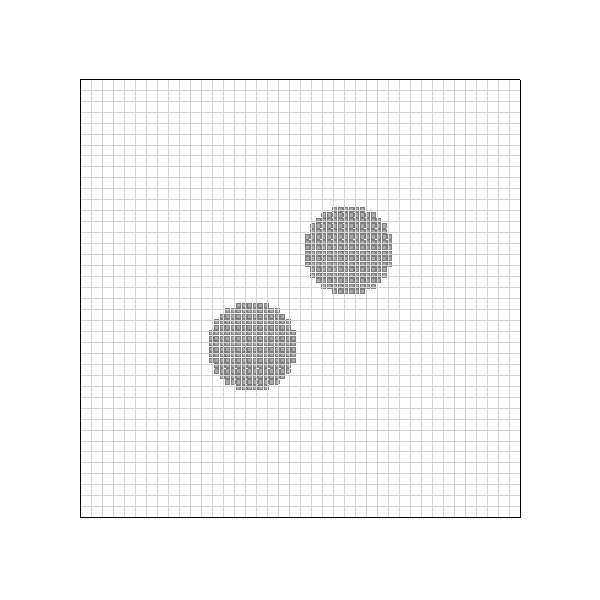
\includegraphics[width=0.2\textwidth]{./PICS/EDC2.pdf}}
\subfloat[$t=2.25$]{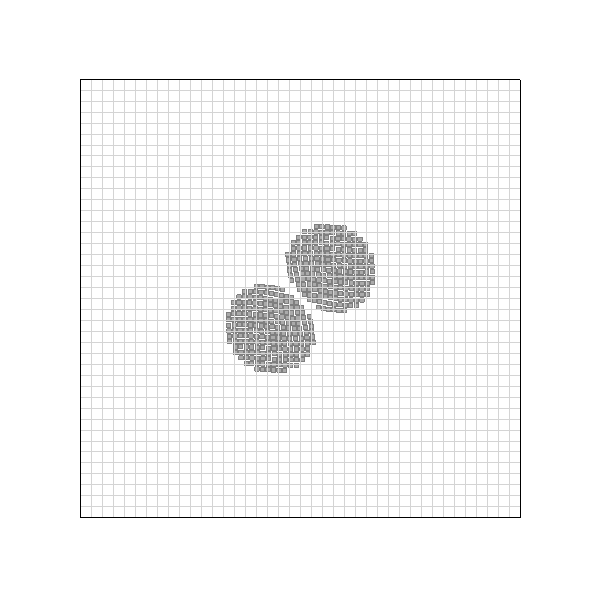
\includegraphics[width=0.2\textwidth]{./PICS/EDC3.pdf}}
\subfloat[$t=3.1$]{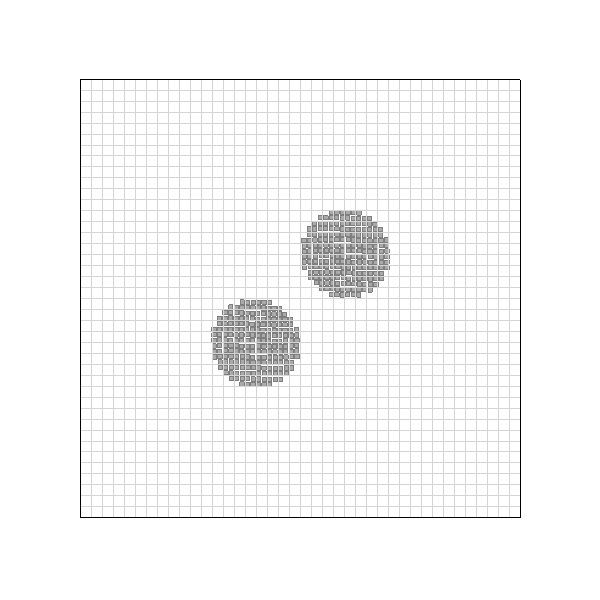
\includegraphics[width=0.2\textwidth]{./PICS/EDC4.pdf}}
\caption{Disks motion at various instants of time}
\label{Fig:TestCaseEDC_Res1}
\end{figure}

Figures~\ref{Fig:TestCaseEDC_Res2}(a) and (b) show the evolution of the energies with time calculated using linear hat and cubic spline shape functions. At initial time and till the time of collision, there is only kinetic energy for both the disks due to the initial velocities. 

\begin{figure}[h]
\subfloat[Linear hat shape function]{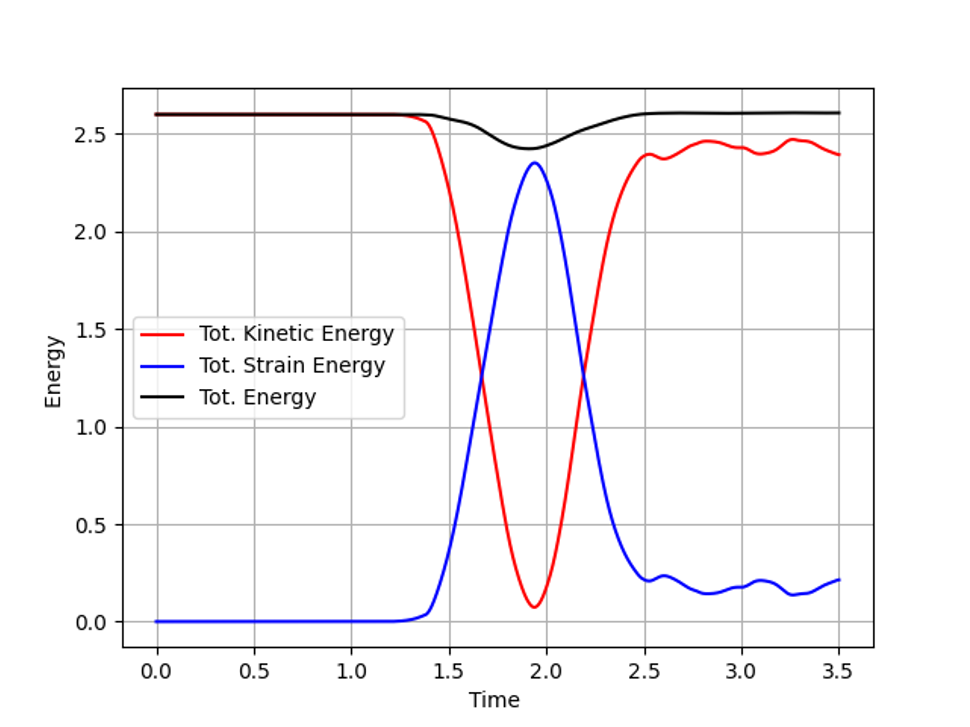
\includegraphics[width=0.35\textwidth]{./PICS/EDC_Energy_LH.png}}
\subfloat[Cubic spline shape function]{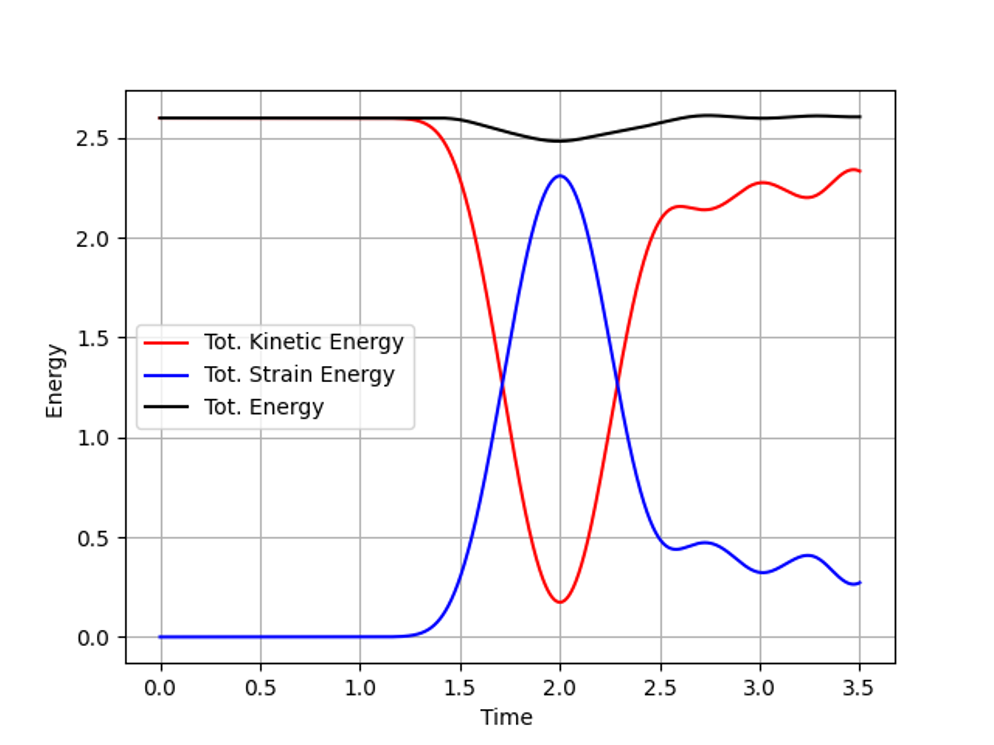
\includegraphics[width=0.35\textwidth]{./PICS/EDC_Energy_CS.png}}
\caption{Evolution of the kinetic, strain and total energies of the disks}
\label{Fig:TestCaseEDC_Res2}
\end{figure}

Once the disks collide, a portion of the total energy is converted to strain energy. Since there are no dissipative mechanisms modeled in this problem, the total energy of the disks should be conserved. Both the linear hat and the cubic spline shape function is able to recover the total energy completely. A temporary loss of total energy is observed during the time of collision. This is due to the mass lumping algorithm adopted which tend to make the solution slightly dissipative. The exact time of contact happens at time $t=1.58$sec while the numerical simulations tend to predict the contact much early. This is because, the contact in MPM occurs through the background grid nodes and not through material points. This inaccuracy can be reduced by refining the background grid further.

\subsection{Dam break simulation}
To demonstrate the application of \Ex solver to simulate flow of fluids, dam break simulation is carried out. The test case consists of a column of water of height $H_0$ and width $L_0$ located inside a square domain, at time $t=0$. For $t>0$, the water column is left free and flows down due to gravity. Water fills up the entire domain as time progresses. Experimental measurement of the water front is available \cite{martin1952} for comparison with MPM results. 

For MPM simulations, the domain is chosen as shown in Figure~\ref{Fig:TestCaseDB}(b). A square domain of side 0.4m is chosed for creating the background grid. The square grid is descretized using 100 cells in each direction. The height of the water column is chosen as 0.2m and the width as 0.1m. Contrary to the previous test cases discussed, water is treated as a fluid and requires specification of an equation of state. In this study, water is modelled using a barotopic equation of state that relates pressure to the density of water as,
\begin{align}
p=\kappa\left[\left(\frac{\rho}{\rho_0}\right)^\gamma-1\right]
\end{align}
The value of $\kappa$ and $\gamma$ is set as 20000 and 7.0 respectively. The density of water is initialised as 1000 kg/m3. Simulation is performed using $CFL=0.1$ and $\alpha_{P-F}=0.95$. The spatial descretization scheme used is that of cubic-spline. The simulation snapshot at various instants of time as shown in Figure~\ref{Fig:TestCaseDB_Res1}. 


\begin{figure}[tbh]
\subfloat[Problem definition of dam break test case]{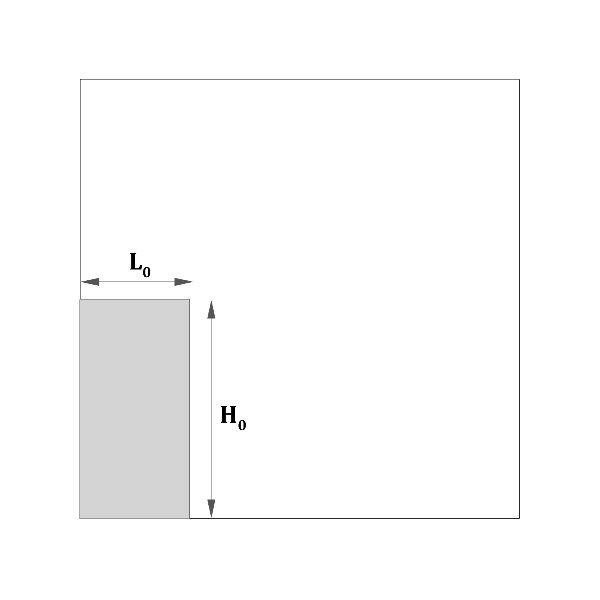
\includegraphics[width=0.4\textwidth]{./PICS/DB_PDT.pdf}}
\subfloat[MPM modeling of dam break case]{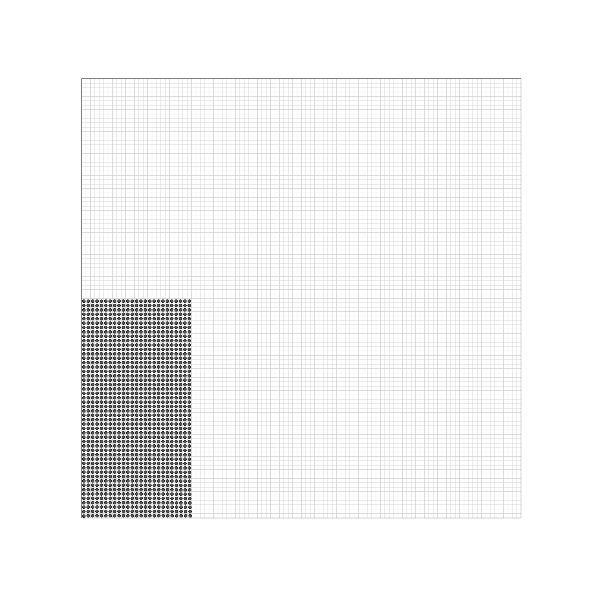
\includegraphics[width=0.4\textwidth]{./PICS/DB1.pdf}}\\
\caption{Dam break test case}
\label{Fig:TestCaseDB}
\end{figure}

\begin{figure}[h]
\subfloat[$t=0.0$]{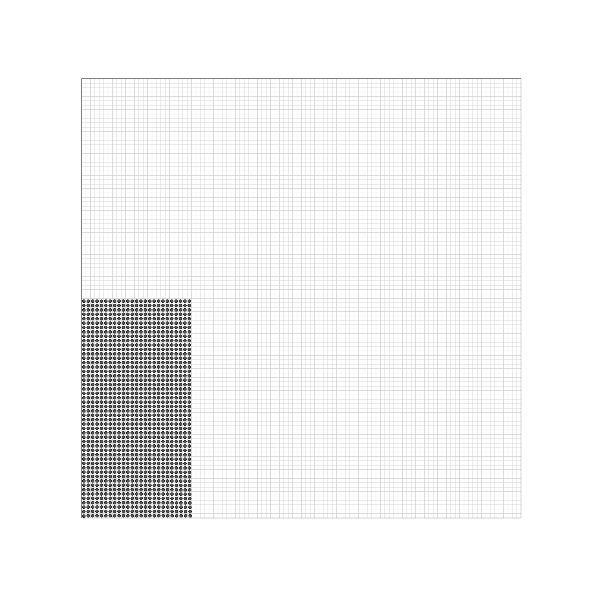
\includegraphics[width=0.25\textwidth]{./PICS/DB1.pdf}}
\subfloat[$t=0.15$]{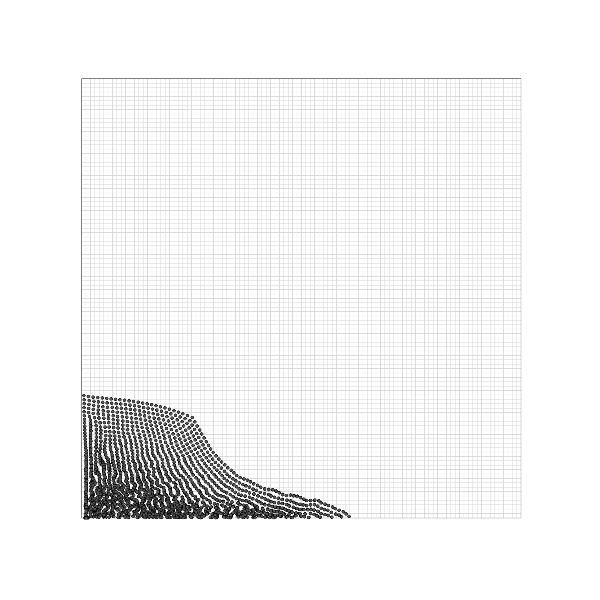
\includegraphics[width=0.25\textwidth]{./PICS/DB2.pdf}}
\subfloat[$t=0.22$]{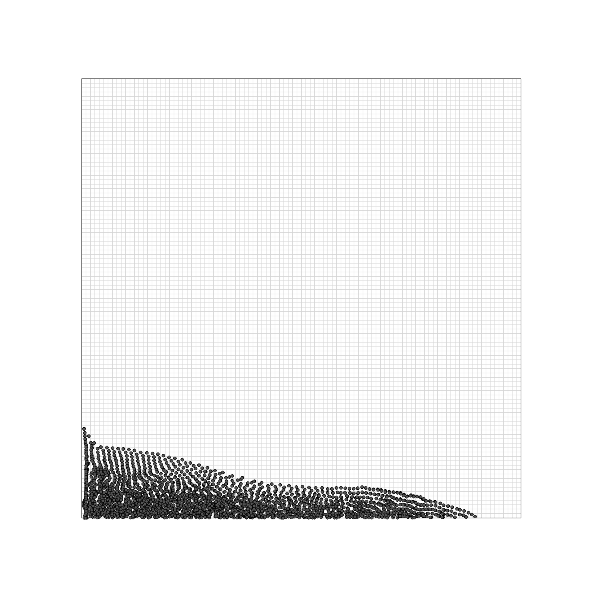
\includegraphics[width=0.25\textwidth]{./PICS/DB3.pdf}}
\subfloat[$t=0.29$]{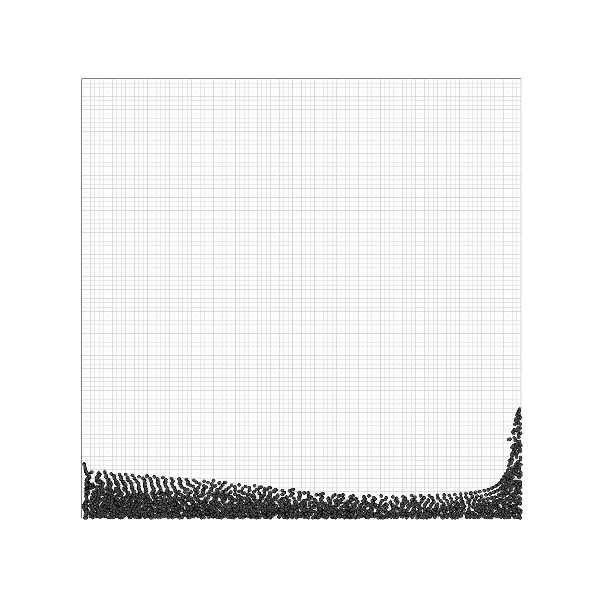
\includegraphics[width=0.25\textwidth]{./PICS/DB4.pdf}}
\caption{Water front movement at various instants of time}
\label{Fig:TestCaseDB_Res1}
\end{figure}

Figure~\ref{Fig:TestCaseDB_Res2} shows a comparison of the water front calculated using \Ex and experimentally obtained water front values \cite{martin1952} at various times. A good comparison is obtained between the numerical and experimental values thereby validating the solver.

\begin{figure}[h]
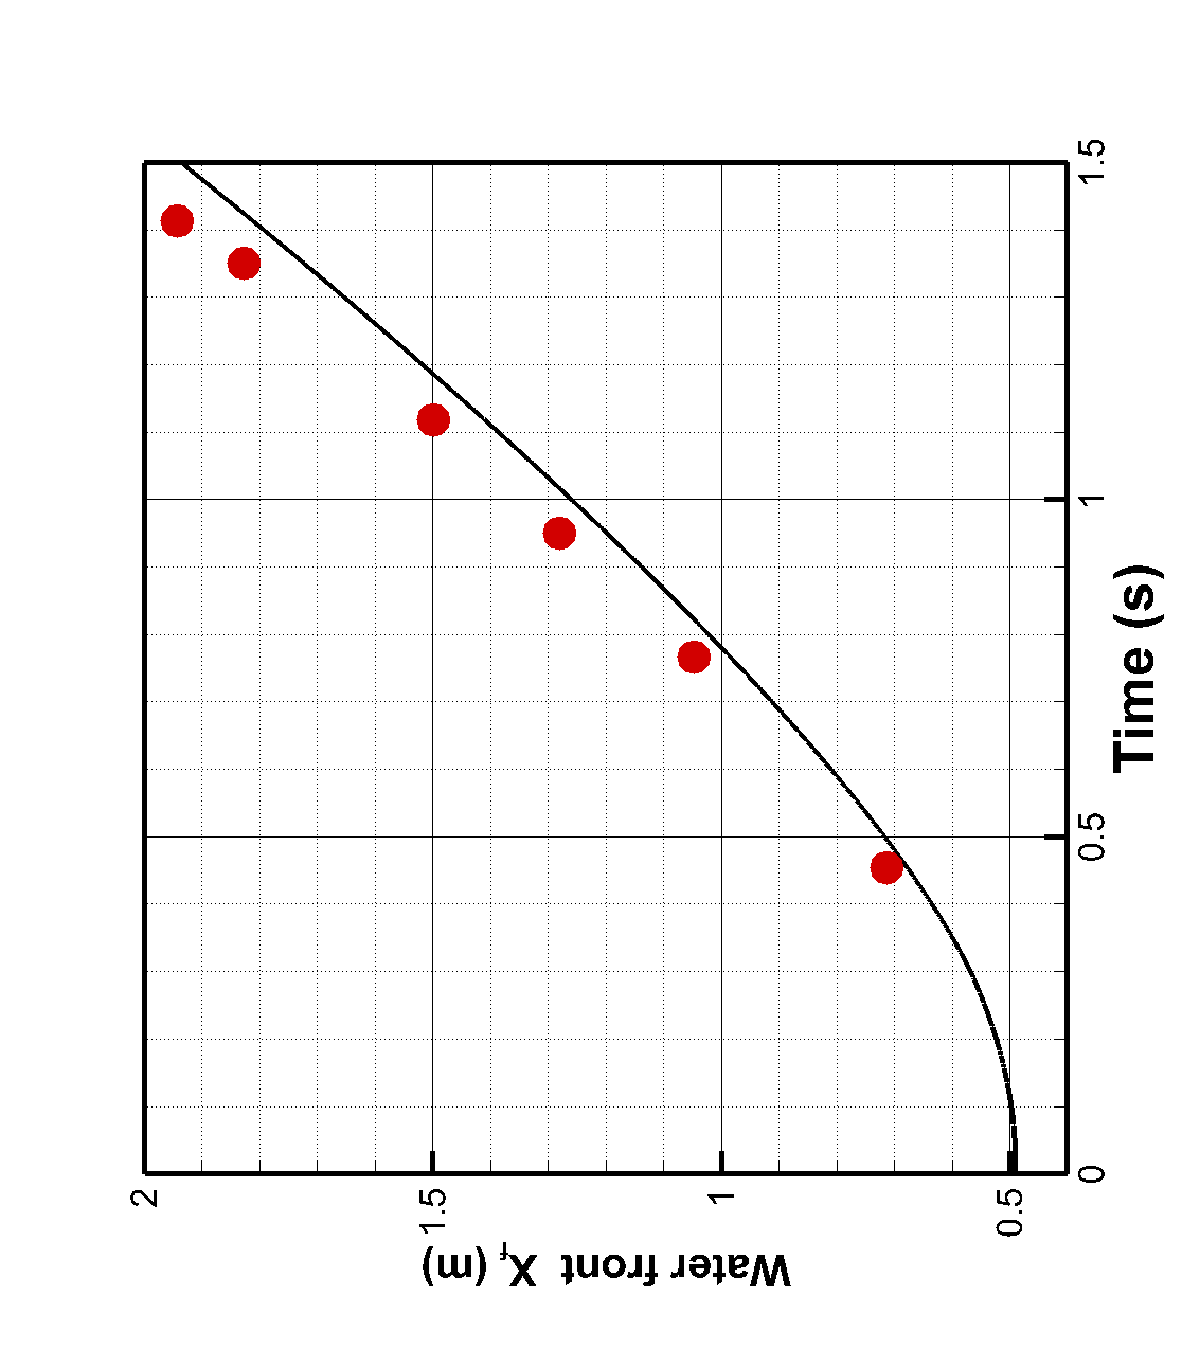
\includegraphics[width=0.4\textwidth, angle =-90]{./PICS/DB_Res2.pdf}
\caption{Time evolution of water front location. Line is MPM solution and circles indicate experimental data from \cite{martin1952}}
\label{Fig:TestCaseDB_Res2}
\end{figure}

\section{Results}
The application of the \Ex MPM solver to simulate membrane compaction is discussed in this section. 

%A few words about the experiments
The membrane compaction experiment to be simulated in MPM is chosen from \cite{WU2022115875}. In the cited article, the authors have chosen an HPRO (XUS1818, Dupont Water Solutions, Edina, Minnesota, USA) membrane to perform experimental studies on its flux and salt rejection properties. The membrane is subjected to high (14 bar) and ultra-high pressures (200 bar) using pressurized N2 gas. After the application of pressure, a sample of the membrane is analyzed for its pore structures in an SEM. The original and compressed membrane heights are available for MPM validation.

%Modeling challenges.
One of the primary challenges in modeling the membrane compaction experiment using MPM is to obtain the initial material point locations. Due to the intricate and minute pore structures, detailed computer-aided modeling of the membrane is next to impossible. In this study, the initial material points are generated  from the images obtained from SEM. Already existing Python modules are used to read the SEM image file. Once the image file is read by the python script into an array, it is converted into grayscale. Since the objective here is to identify and represent only the larger microvoids in the membrane, image intensity-based filtering is performed. Based on trial and error, the image is clipped between intensities $20$ and $180$ to obtain a good representation of the membrane. Each pixel in the clipped image is then treated as a material point. The dimensions of the membrane are calibrated such that the entire membrane height is kept close to 50 microns. For ease of computation, the membrane geometry is assumed to be periodic, and only one layer of material points is retained in the third dimension. The top row in Figure~\ref{fig:expt_mpm_compare} shows the SEM image and the material point locations used in this study.

\begin{figure}[tbh]
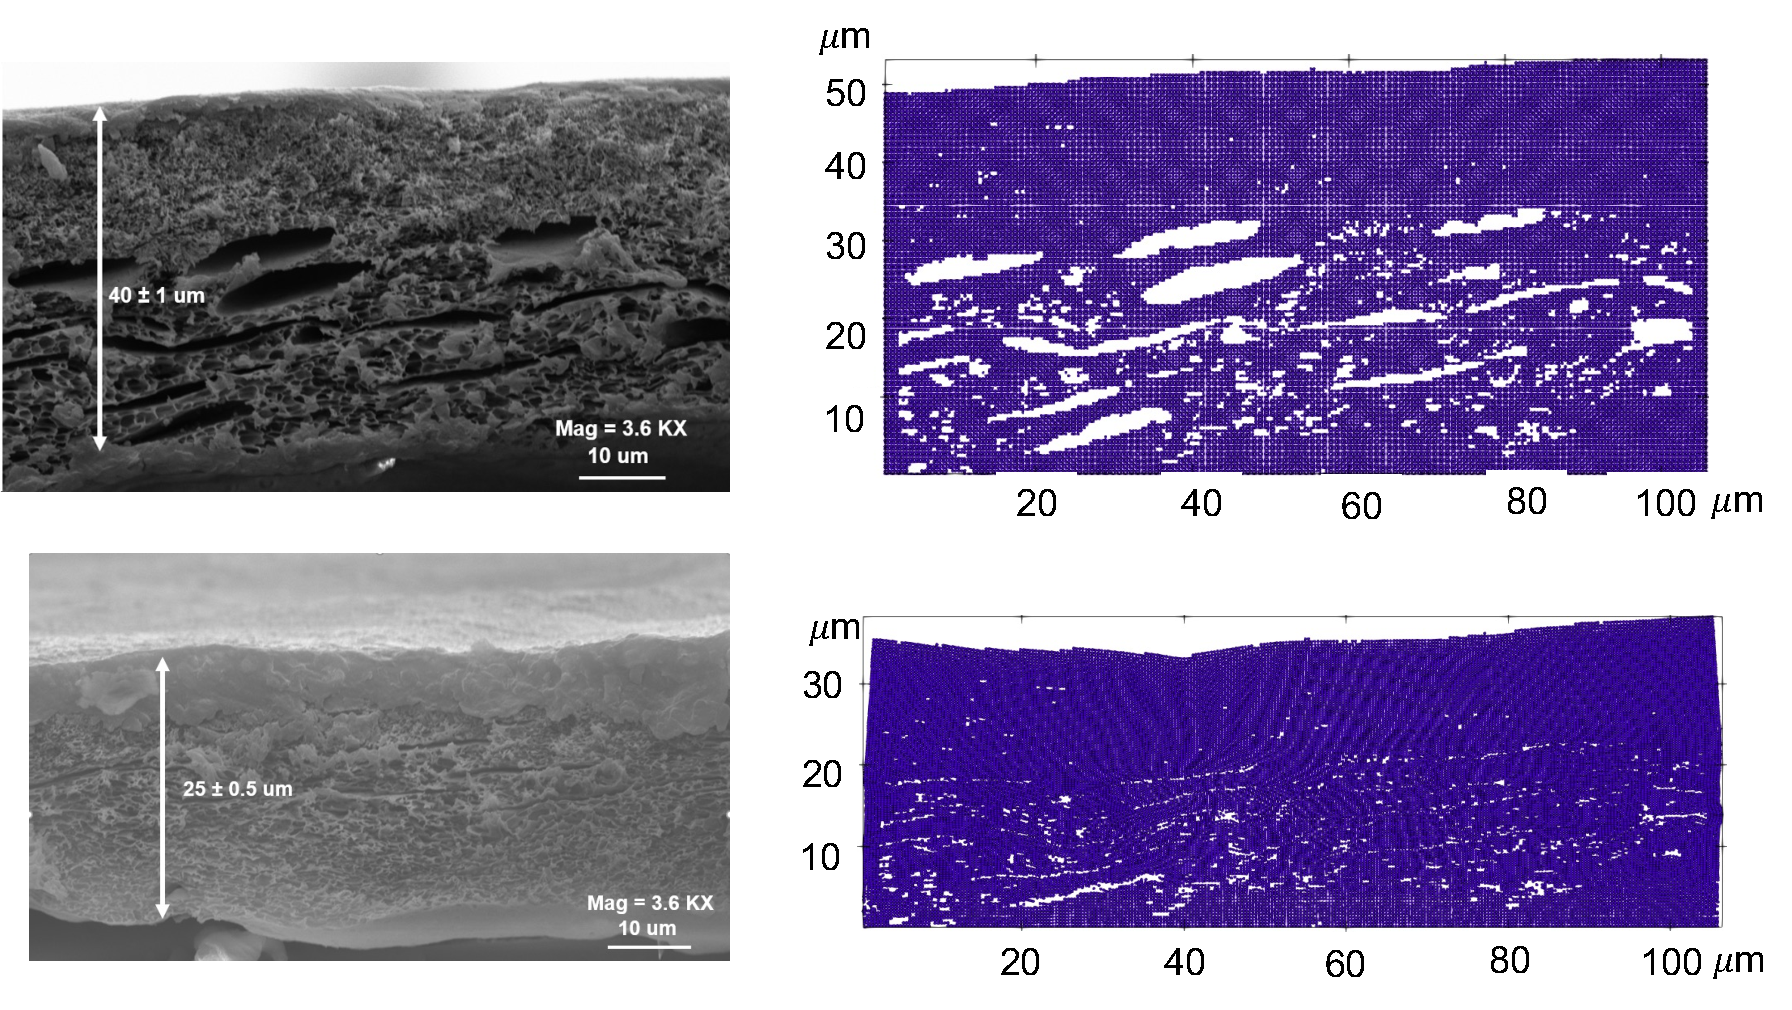
\includegraphics[width=\textwidth]{./PICS/compare_expt_mpm.pdf}
\caption{(top left) and (top right) show SEM image of PSF layer and corresponding material point representation that is used as initial condition for our simulations. (bottom left) and (bottom right) show SEM image of compressed PSF layer at 200 bar pressure and corresponding snapshot of material points at steady state for a compression simulation at 200 bar.}
\label{fig:expt_mpm_compare}
\end{figure}

%Problem setup
The PSF material in the membrane is modeled as a linear elastic material. The value of Young's modulus (134 MPa) is obtained from a tensile test carried out at the UCLA NanoMeTeR laboratory, and the Poisson's ratio is assumed to be $0.3$. The application of pressure (200 bar) on the membrane is modeled by applying a fictitious body force on the material points. The applied body force is calibrated such as to obtain an average normal stress equal to the imposed pressure. The boundary condition applied on the bottom surface of the background grid is that of a no-slip wall, while slip walls are applied on all the other boundaries. To maintain a low computational cost, the linear-hat function is used as the spatial scheme. The values of CFL and $\alpha_{P_F}$ are set as $0.1$ and $0.95$, respectively.


%
%Results
Simulation is carried out in an HPC environment with 2 GPU nodes. Figure~\ref{fig:stress}(a) shows the time evolution of the average normal stress in the y-direction on the top surface. It can be observed that the stress value recovers to  that of the imposed pressure indicating that the steady-state solution is attained. The bottom images in Figure~\ref{fig:expt_mpm_compare} show a comparison between the experimentally and numerically observed compacted membrane and their pore structure. Experiments report a membrane deflection of 15 microns (a strain of 0.375) while MPM results show a deflection of 17 microns (a strain of 0.34). An accurate prediction in terms of deflection is obtained with the deviation of MPM results from experiments being only 3.5\%. Figure~\ref{fig:stress}(b) shows the y-normal stress and the compacted configuration of the membrane. The figure shows the presence of microvoids now compressed under pressure, very similar in shape to that found in experiments. Regions of stress concentrations near the corners of the voids can also be observed.

\begin{figure}[tbh]
\centering
\begin{subfigure}[b]{0.49\textwidth}
    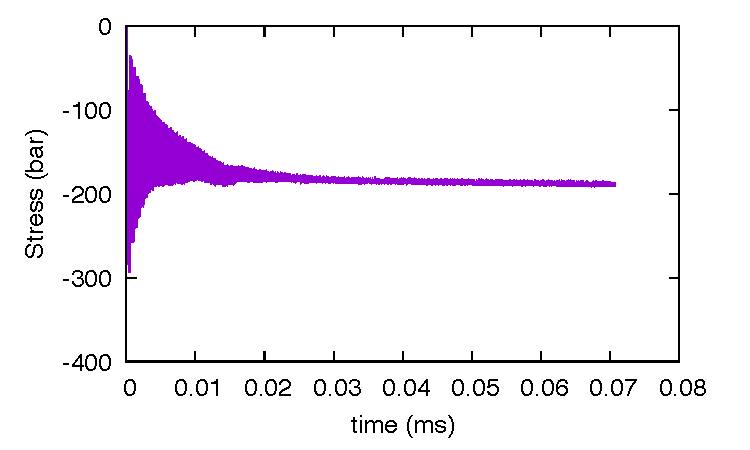
\includegraphics[width=0.99\textwidth]{./PICS/force.pdf}
    \caption{}
\end{subfigure}
\begin{subfigure}[b]{0.49\textwidth}
    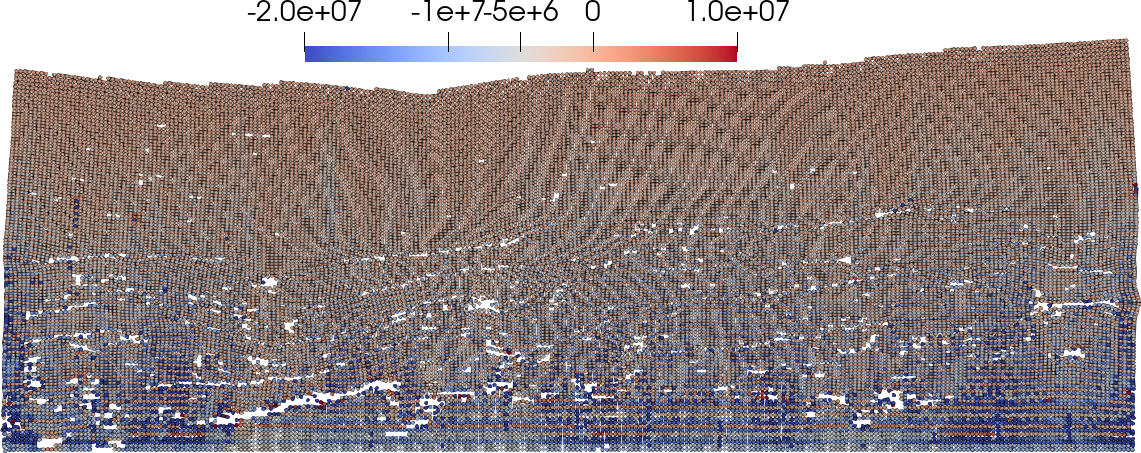
\includegraphics[width=0.99\textwidth]{./PICS/stress.png}
    \caption{}
\end{subfigure}
\caption{(a) average axial stress history at the bottom of the domain that tends to 200 bar at steady-state and (b) is the stress distribution in Pa among material points at steady-state.}
\label{fig:stress} 
\end{figure}
\section{Conclusions}
\newpage{}
\bibliography{refs}
%\bibliographystyle{unsrt}
%
\end{document}
